\chapter{Introduction}\label{chap:intro}
\newpage
\sloppy

Neurosurgical procedures such as deep brain stimulation (DBS) involve targeting small, deep brain structures where spatial deviations of only 1 to 2 millimeters (mm) can be the difference between optimal therapeutic efficacy and adverse effects \cite{Horn2018-qq}. This level of precision highlights a fundamental challenge in neuroimaging: the need for millimetric localization of brain structures despite inter-individual anatomical variability, differences across imaging modalities, imaging artifacts, and imaging sessions.

Precise localization of brain structures remains challenging using clinical neuroimaging \cite{Boutet2021-vg}. Some targets may be difficult to locate due to their small size, limited contrast, susceptibility to artifacts, or inter-individual anatomical variability \cite{Lau2020-dh}. Manual localization can be time consuming and subject to observer variability \cite{Miller2023-ct}. Additional tools are needed to improve accuracy, especially in applications that span imaging modalities, populations, and clinical contexts. Recent developments in machine learning (ML) offer opportunities to address challenges in brain structure localization by improving accuracy, automation, and scalability \cite{Andrews2025-kd}.

This dissertation leverages brain coordinates and ML to develop an open software infrastructure that supports spatially precise and interpretable workflows in neuroimaging and neurosurgery. We investigate how ML-driven brain landmark localization can support millimetric image alignment quality control, enhance surgical targeting workflows, and facilitate population-level morphometric analysis.

In this introductory chapter, we begin with a historical overview of stereotactic neurosurgery and the development of coordinate-based targeting. We present the foundations of magnetic resonance imaging (MRI) and highlight advances in acquisitions, including ultra-high-field MRI. A brief overview of image registration is also discussed, followed by an introduction of coordinate-based frameworks for quantifying alignment and modeling brain structure. Finally, we discuss ML algorithms relevant to this dissertation and outline recent advances to improve the automation and scalability of brain structure localization.

\section{Stereotactic Neurosurgery}
\label{sec:SNSX}
Stereotactic neurosurgery is a subspecialty of neurosurgery dedicated to targeting brain structures for diagnostic or therapeutic purposes. The word stereotaxy is derived from the Greek words “stereos-”, for three-dimensional (3D), and “-taxy”, for arrangement first used by Horsley and Clarke in 1908 \cite{Horsley1908-om}. Central to this approach is the accurate localization of intracranial targets within a standardized 3D space. Early stereotactic innovations (Figure \ref{fig:ch1_Figure_stereoframe}) enabled clinicians and researchers to consistently identify, compare, and intervene in specific regions of the brain, which is central to many brain mapping applications.

\begin{figure}[hbt!]
    \centering
    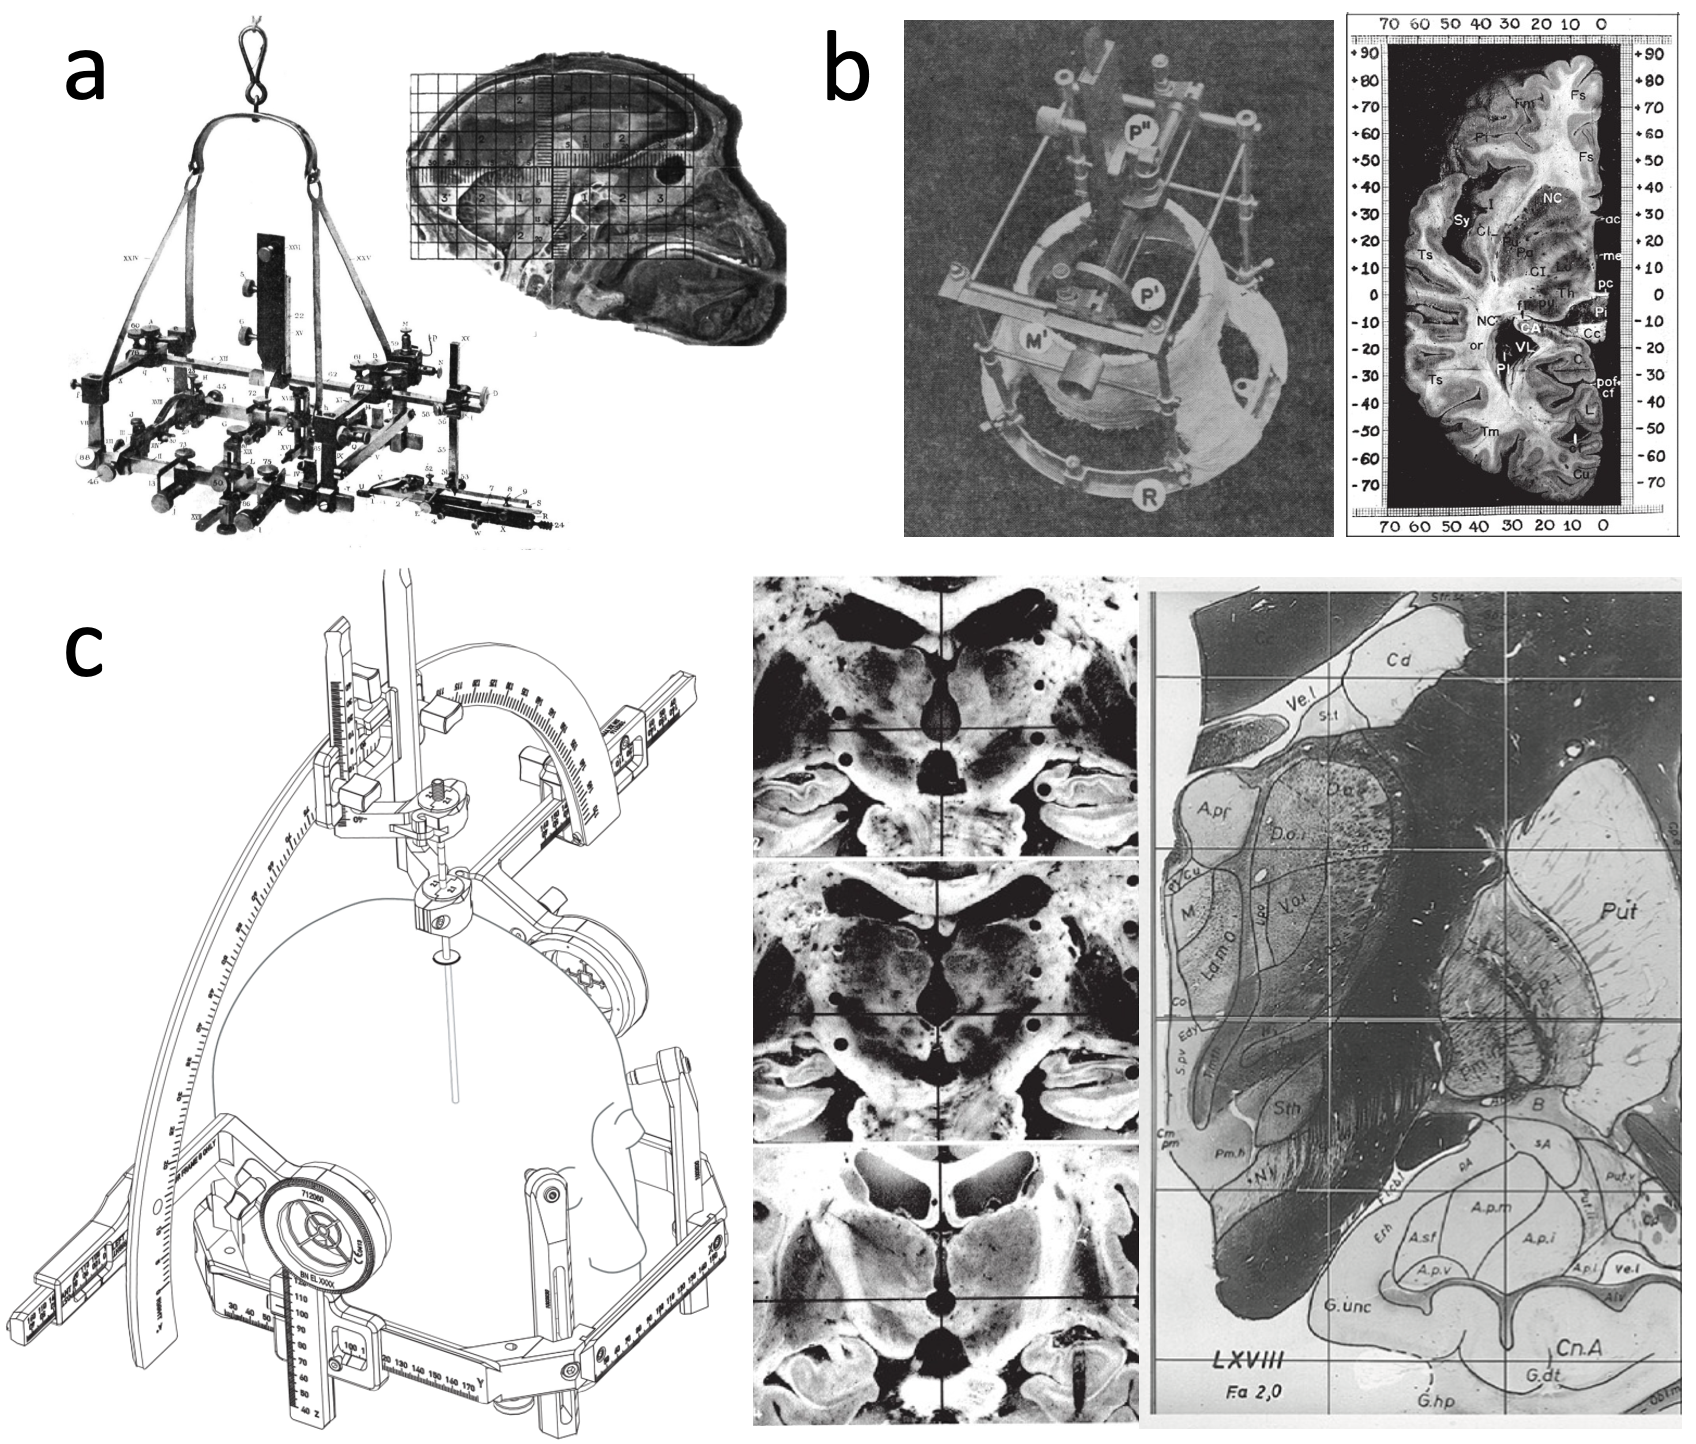
\includegraphics[width=0.85\linewidth]{figs/ch1_Figure_stereoframe2.png}
    \caption{Key innovations in stereotactic neurosurgery and their associated reference spaces. (a) Horsley and Clarke’s \cite {Horsley1908-om} frame for cerebellar research, shown with their accompanying atlas. (b) Model V, the frame by Spiegel and Wycis \cite{Spiegel1947-rq} for human brain interventions, alongside their post-mortem reference brain. (c) Modern Leksell-style frame used in clinical practice, shown with common atlases such as Talairach \cite{Talairach1957-eb} and Schaltenbrand \cite{Schaltenbrand1977-ge}.}
    \label{fig:ch1_Figure_stereoframe}
\end{figure}

\subsection{Overview of Stereotactic Neurosurgery}
Victor Horsley and Robert Clarke introduced the first stereotactic apparatus for experimental neurophysiology in non-human primates \cite{Horsley1908-om}. Their system employed a Cartesian coordinate frame anchored to external cranial landmarks, allowing for reproducible access to deep brain structures and marking the first formal application of spatial coordinate systems in neuroscience (Figure \ref{fig:ch1_Figure_stereoframe}a).

While Horsley and Clarke alluded to the use of the apparatus in humans, it was in 1947 that Ernest Spiegel and Henry Wycis introduced the first stereotactic apparatus for human neurosurgery \cite{Spiegel1947-rq}. Their system, called Model V (Figure \ref{fig:ch1_Figure_stereoframe}b), employed a Cartesian coordinate frame which leveraged internal cerebral landmarks. This innovation enabled targeting of subcortical structures, facilitating interventions for movement disorders, psychiatric conditions, and pain management. Building upon their foundation, Lars Leksell developed the first arc-centered stereotactic system in 1949 \cite{Leksell1949-wl}, introducing a polar coordinate approach that enhanced surgical flexibility and precision (Figure \ref{fig:ch1_Figure_stereoframe}c).

A major advancement in intracranial localization came with the identification of internal anatomical landmarks. Jean Talairach observed that the anterior commissure (AC) and posterior commissure (PC) could be reliably visualized using pneumoencephalography \cite{Dandy1918-os}, an imaging technique involving the injection of air into the ventricular system, and used it as a central axis for stereotactic navigation \cite{Talalrach1957-bs}. Talairach’s early work in the 1950s introduced the concept of a proportional grid system anchored to the AC–PC line (Figure \ref{fig:ch1_Figure_templates}a), which was later formalized in the 1988s as the co-planar stereotactic atlas developed with Pierre Tournoux \cite{Talairach1988-wk}. Although based on a single postmortem brain, the Talairach atlas provided a reproducible framework for reporting intracranial coordinates. It shifted the field away from reliance on external skull landmarks and toward internal anatomical geometry.

\begin{figure}[hbt!]
    \centering
    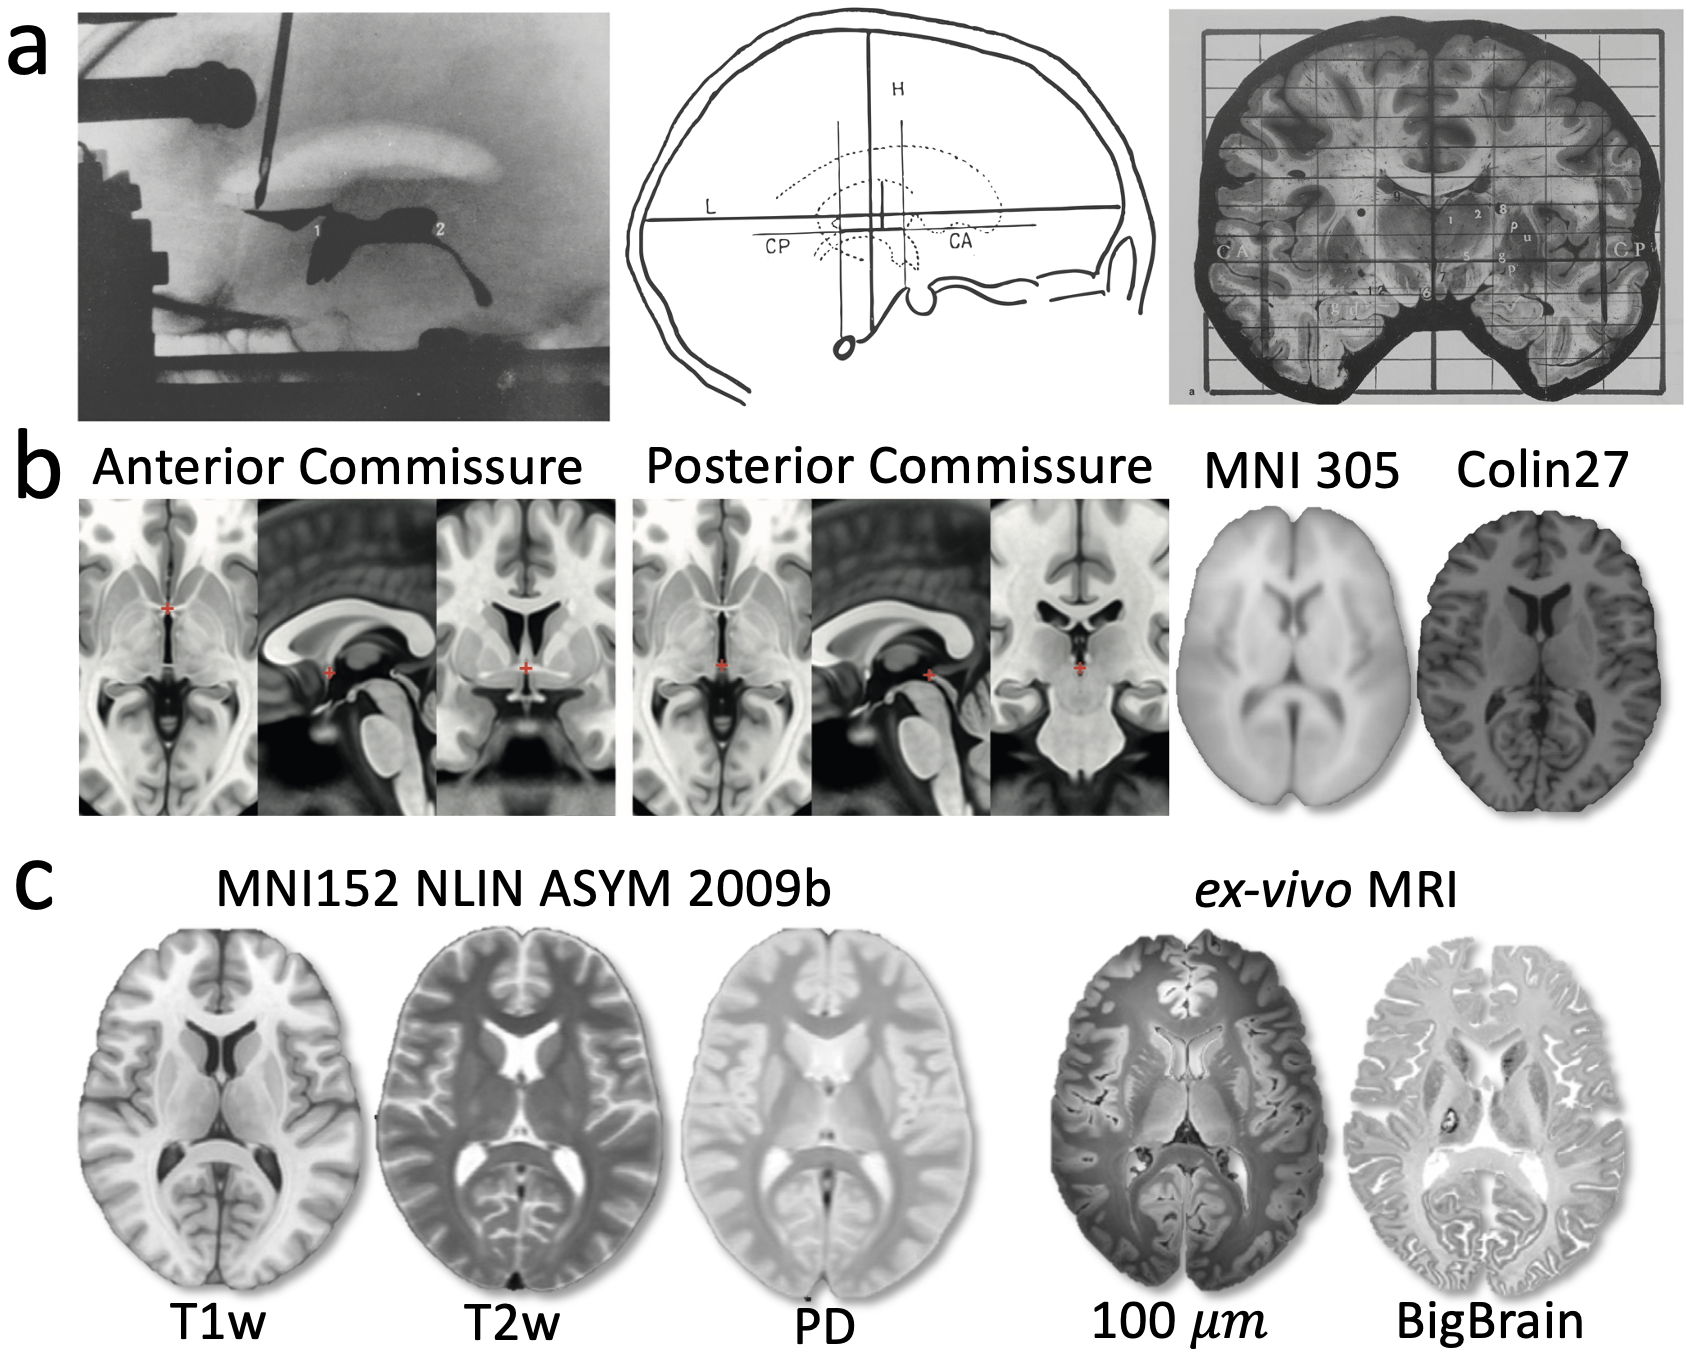
\includegraphics[width=0.86\linewidth]{figs/ch1_Figure_templates2.png}
    \caption{Emergence of Stereotactic Spaces. (a) Classical Talairach space defined by stereotactic landmarks \cite{Talairach1957-eb}. (b) Early MRI-based average brain created in Talairach space \cite{Collins1994-dx}. (c) Modern templates \cite{Fonov2011-ck,Edlow2020-mo, Amunts2013-vu} improved using nonlinear registration.}
    \label{fig:ch1_Figure_templates}
\end{figure}

These early innovations established the foundation for population-based brain templates that emerged with the advent of MRI (see Section~\ref{sec:MRI}). The Montreal Neurological Institute (MNI) developed average brain templates derived from multiple individuals, enabling more representative spatial normalization across subjects. An important example is the MNI305 template \cite{Collins1994-ue}, which leveraged manually defined stereotactic landmarks (i.e., AC and PC) to align MRI scans of 305 individuals, approximating the Talairach space. This marked a convergence between classical stereotactic principles and neuroimaging, allowing more representative spatial normalization between subjects (Figure \ref{fig:ch1_Figure_templates}b). Since then, further improvements in nonlinear image registration (see Section~\ref{sec:registration}) have culminated in brain templates \cite{Fonov2009-oi} that preserve anatomical detail and support more accurate inter-subject alignment (Figure \ref{fig:ch1_Figure_templates}c).

Today, stereotactic spaces underpin a wide range of neuroimaging applications, from structural and functional mapping to large-scale meta-analyses \cite{Yarkoni2011-sr,Dockes2020-nw}. These frameworks facilitated the development of shared databases that encompass anatomical, cytoarchitectonic, and functional information \cite{Eickhoff2005-qb}. Despite advances in non-invasive neuroimaging and image registration, fundamental stereotactic principles remain central to both neurosurgical navigation and brain mapping.

\subsection{Deep Brain Stimulation}
Deep brain stimulation (DBS) is a stereotactic procedure that involves the targeted implantation of electrodes into deep brain nuclei to modulate dysfunctional neural circuits. Since its formal introduction by Alim Benabid in the late 1980s \cite{Benabid1987-mp}, DBS has revolutionized the management of various neurological disorders by providing a reversible, adjustable, and less destructive alternative to lesion-based surgeries \cite{Limousin1990-oz,The-Deep-Brain-Stimulation-for-Parkinson-s-Disease-Study-Group2001-ss}. To date, DBS has been implanted in over 250,000 patients worldwide \cite{Schulder2023-aj}, primarily for the treatment of movement disorders such as Parkinson's disease (PD), essential tremor, dystonia, and Tourette’s syndrome, as well as for select psychiatric conditions including obsessive-compulsive disorder and treatment-resistant depression \cite{Lozano2019-dv}.

The subthalamic nucleus (STN) is the most commonly targeted structure in DBS for PD \cite{Lozano2019-dv}. This lens-shaped nucleus (Figure \ref{fig:ch1_Figure_whymm}, roughly 10 mm in length, is located inferior to the thalamus, adjacent to the substantia nigra and lateral to the red nucleus (RN) \cite{Prasad2024-hi}. The STN acts as a major relay within the basal ganglia (BG) \cite{DeLong2007-cv}. It receives convergent cortical, pallidal, and thalamic inputs and is involved in regulating motor output within the BG circuit \cite{DeLong2007-cv,Jeon2022-wg}. Due to its integrative role, DBS of the STN results in significant motor improvements \cite{Hermann2024-tr}-but also in unwanted side effects if adjacent fiber tracts or nearby structures are inadvertently activated \cite{Kiss2007-mu,Reich2022-jf}.

Despite widespread clinical use, the therapeutic mechanisms of DBS remain poorly understood. Initial theories proposed a “functional lesion” effect, where high-frequency stimulation inhibits overactive neurons locally \cite{Benabid1987-mp, Benabid1996-jd}. DBS can also be viewed as a network-level modulator, capable of reshaping oscillatory activity and restoring information flow across distributed brain networks \cite{Miocinovic2013-rs,Herrington2016-xr}. The therapeutic effects vary by condition and symptom: tremor may improve within seconds, whereas benefits in dystonia or depression can take weeks to months, suggesting additional contributions from synaptic plasticity and long-term network reorganization \cite{Ashkan2017-hb}. These insights support an expanded view of DBS as a dynamic intervention capable of reshaping dysfunctional brain circuits over multiple timescales.

\subsection{Why millimeters matter}
\label{sec:whymm}
Achieving therapeutic benefit from DBS requires the millimetric implantation of electrodes. While stereotactic neurosurgery has embraced the need for accuracy, DBS uniquely amplifies this demand due to three converging factors: (1) the small size of target structures, (2) their complex anatomical context, and (3) the highly localized nature of stimulation effects.

DBS targets such as the STN, globus pallidus internus, and ventral intermediate nucleus are a few millimeters in size. Within these already small structures, stimulation is often directed at even smaller subregions that are functionally specialized. In the case of the STN, for example, different functional subzones are associated with distinct symptom domains, ranging from motor control to mood and behavior \cite{Hollunder2024-wc}. Hence, the STN is a DBS target for a range of neurological and psychiatric conditions, including PD \cite{Deuschl2006-ar}, dystonia \cite{Ostrem2017-rw}, Tourette’s syndrome \cite{Mallet2008-ky}, and obsessive-compulsive disorder \cite{Dai2022-uy}. These therapeutic zones are in close proximity to each other, so even a 1-2 mm deviation in electrode placement can shift stimulation to less effective or potentially adverse area \cite{Akram2017-ru}.

DBS targets are located within an anatomically crowded and heterogeneous environment. The subcortex is traversed by multiple orthogonal and intersecting fiber tracts, with neighboring structures often fulfilling opposing or unrelated functions. For example, the internal capsule lies adjacent to the STN and carries motor fibers from the cortex; inadvertent stimulation here can cause contractions or dysarthria \cite{Tripoliti2011-ca}. Similarly, stimulation that extends into associative or limbic territories of the STN may alter cognition or emotion \cite{Mallet2007-ur}.

\begin{figure}[hbt!]
    \centering
    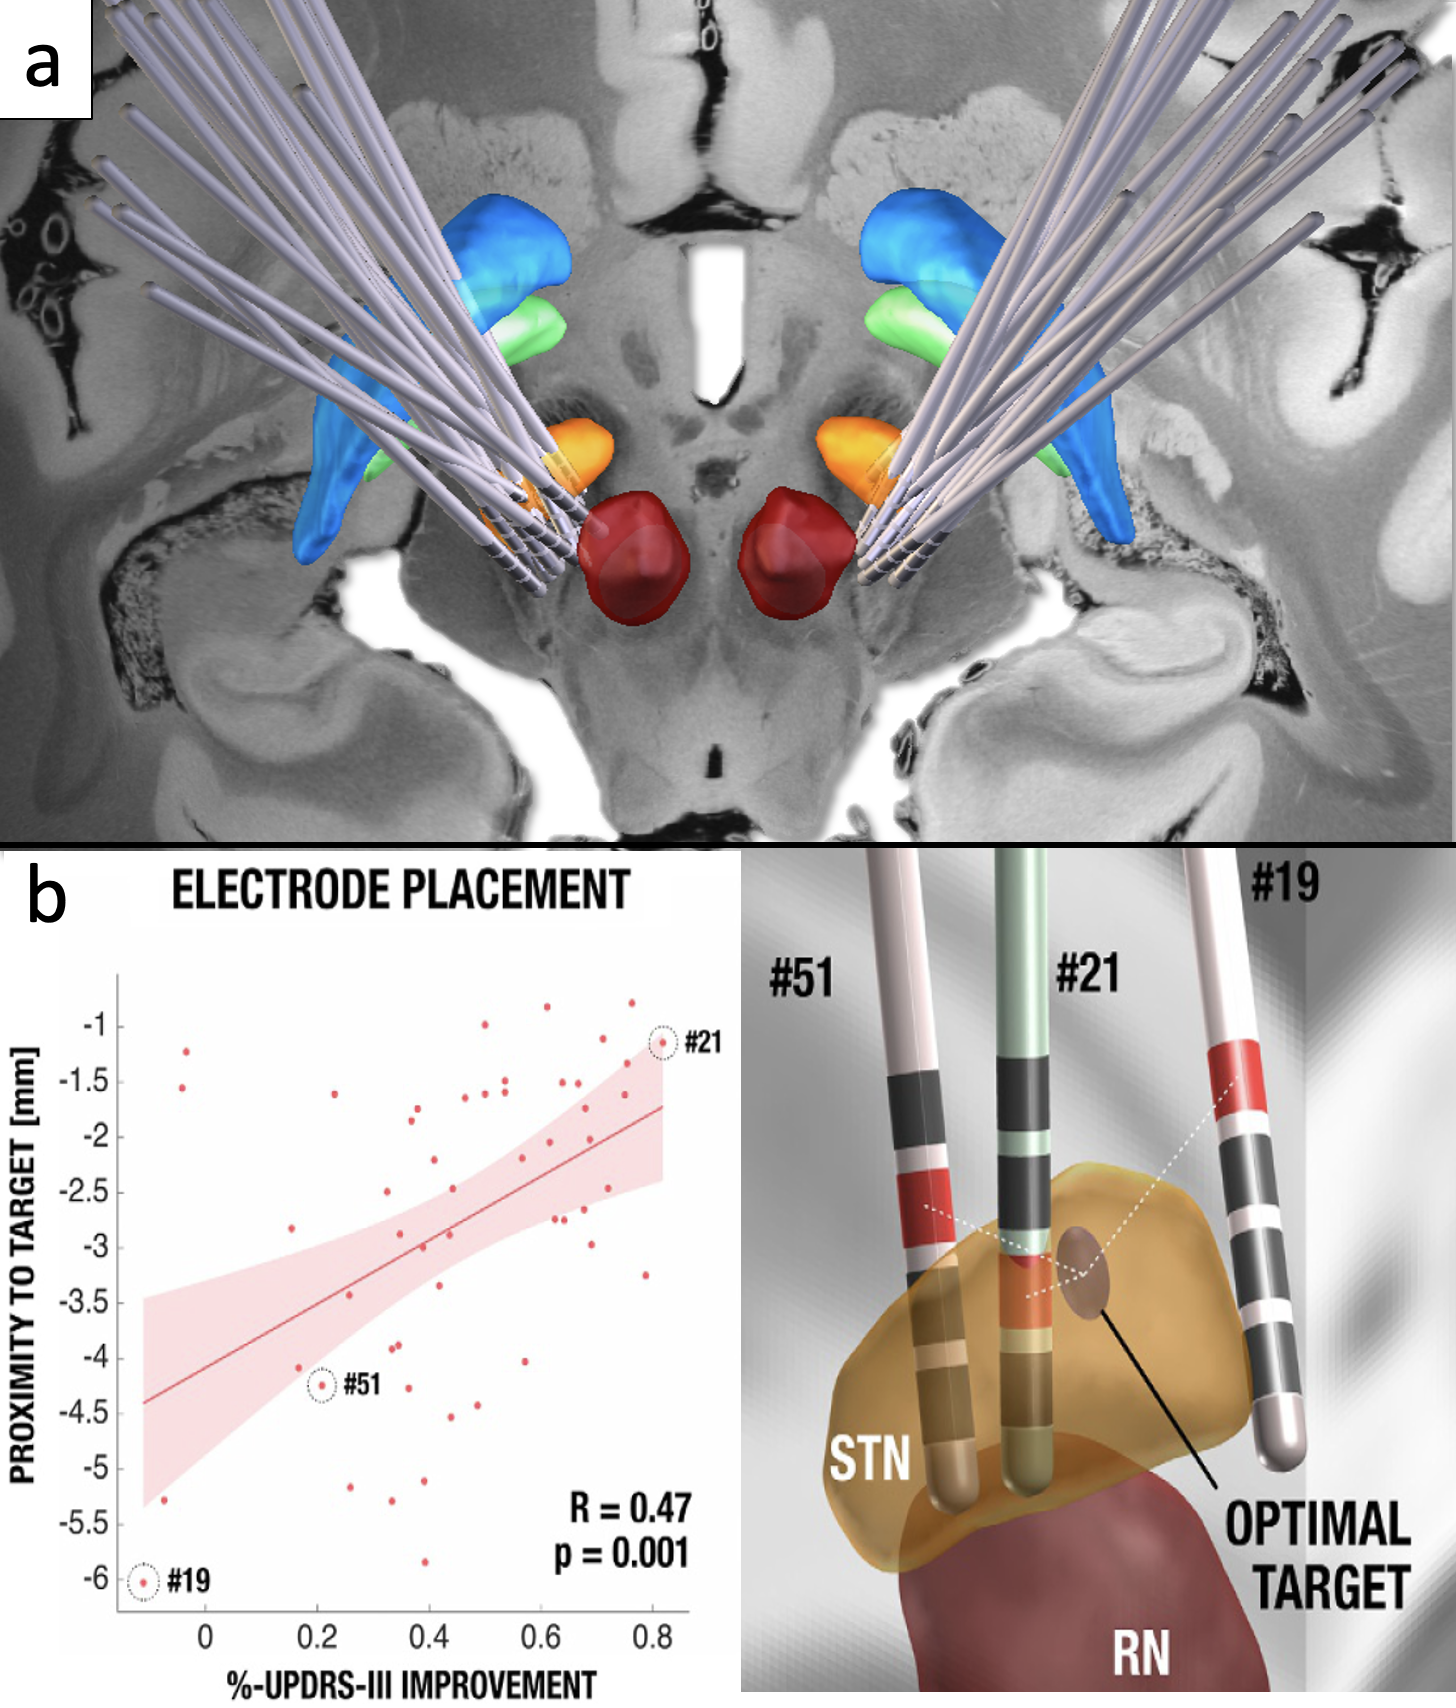
\includegraphics[width=0.97\linewidth]{figs/ch1_Figure_whymm2.png}
    \caption{Why millimeters matter in deep brain stimulation (DBS). (a) Example from a population study showing DBS electrodes warped to a common atlas. (b) Correlation between electrode location and clinical outcome, illustrating how a difference of 2~mm (between patients \#51 and \#21) could correspond to a 60\% difference in therapeutic response. Figure in panel b is modified from an open-access article by \cite{Horn2018-qq}}
    \label{fig:ch1_Figure_whymm}
\end{figure}

Unlike systemic therapies, DBS exerts its effect over a localized volume of tissue, typically within a 1–3 mm radius of the electrode. The “volume of tissue activated” (VTA) depends on factors like stimulation amplitude, pulse width, impedance, and local tissue conductivity \cite{McIntyre2006-wh,Butson2007-bn}. This physical limitation means that even a precisely shaped VTA may fail to engage the intended neural circuits if the electrode is off target. Empirical studies show dramatic differences in clinical outcomes between patients with electrodes separated by as little as 2 mm (Figure \ref{fig:ch1_Figure_whymm}b), underscoring the high spatial gradient of therapeutic response \cite{Horn2018-qq, Maks2009-ci}. Thus, this spatial demand determines the threshold for side effects, stimulation battery usage, and the degree of parameter programming required postoperatively. 

From a surgical standpoint, millimetric accuracy is essential not only for localizing the target but also throughout the DBS electrode implantation process. DBS electrodes may traverse up to 80–100 mm of brain tissue, depending on the entry point and target. Deviations in trajectory may increase the risk of complications such as hemorrhage or unintended tissue damage \cite{Ben-Haim2009-os,Rajabian2023-st}. Maintaining millimetric control over the surgical path is therefore critical to ensuring safe DBS electrode implantation.
 
In summary, the clinical success of DBS hinges on achieving and validating millimetric precision. This imperative has driven the evolution of stereotactic techniques, neuroimaging protocols, and computational tools, all aimed at minimizing spatial error. As such, the millimetric demands of DBS serve as a central challenge and benchmark for any system designed to support neurosurgical targeting.

\section{Magnetic Resonance Imaging}
\label{sec:MRI}
MRI origins trace back to the discovery of nuclear magnetic resonance (NMR) by Felix Bloch and Edward Purcell in 1946, who independently demonstrated that atomic nuclei emit measurable radiofrequency (RF) signals when placed in a magnetic field \cite{Bloch1946-ob, Purcell1946-jd}. Subsequent advances, including the development of pulsed NMR by Ernst \cite{Ernst1990-we} and the proposal of spatial encoding through magnetic field gradients by Ernst and Anderson \cite{Ernst1966-yx}, laid the foundation for imaging applications. In the early 1970s, Paul Lauterbur and Peter Mansfield independently introduced the concepts of spatially resolved magnetic resonance imaging, establishing the principles that would revolutionize biomedical imaging \cite{Lauterbur1973-wf,Mansfield1977-ru}. 

Today, MRI is the diagnostic modality of choice for soft tissue visualization and is routinely used in neurosurgical planning, including DBS. Its flexibility, safety, and ability to generate diverse tissue contrasts have made it indispensable for anatomical localization and trajectory planning. In this section, we first review the key physical principles underlying MRI, then examine specialized MRI techniques employed during DBS, and finally highlight the challenges that limit the effectiveness of MRI in subcortical structure visualization.

\subsection{MRI Physics Fundamentals}

MRI is based on the principles of NMR, where atomic nuclei with non-zero spin, primarily hydrogen protons in biological tissues, absorb and re-emit RF energy when placed in a strong magnetic field. In a static magnetic field \(B_0\), proton spins precess at the Larmor frequency:
\begin{equation}
\omega_0 = \gamma B_0
\end{equation}
where \( \omega_0 \) is the precessional (angular) frequency and \( \gamma \) is the gyromagnetic ratio (approximately 42.58 MHz/T for hydrogen). By transmitting a radiofrequency (RF) pulse at this resonant frequency (the $B_1$ field perpendicular to $B_0$), the net magnetization $M$ of proton spins can be tipped away from alignment with $B_0$, producing a detectable MR signal as the spins precess and relax back to equilibrium. This excitation and subsequent signal emission is the essence of NMR and forms the basis of MRI signal generation.

After excitation, the perturbed spins return to equilibrium through two independent relaxation processes characterized by time constants $T_1$ and $T_2$. The longitudinal relaxation (spin-lattice relaxation) with time constant T1 describes the recovery of the $M_z$ component (along the $B_0$ axis) toward its equilibrium value. The transverse relaxation (spin-spin relaxation) with time constant T2 describes the decay of the $M_{xy}$ component (perpendicular to $B_0$) due to dephasing of spins. Quantitatively, one may write the solutions of the Bloch equations for recovery and decay as:
\begin{itemize}
    \item \textbf{Longitudinal relaxation time} (\(T_1\)): Describes the recovery of the longitudinal component of magnetization, \(M_z\), as it realigns with the static magnetic field \(B_0\) following excitation. The time course of this recovery is governed by:
    \begin{equation}
    M_z(t) = M_0 \left(1 - e^{-t/T_1}\right)
    \end{equation}
    Here, \( M_0 \) represents the equilibrium magnetization—i.e., the maximum net magnetization achievable along the longitudinal axis in thermal equilibrium. It is determined by the strength of the external field \(B_0\), the spin density of the tissue, temperature, and the gyromagnetic ratio. Immediately after RF excitation, \(M_z = 0\), and over time, it asymptotically returns to \(M_0\).

    \item \textbf{Transverse relaxation time} (\(T_2\)): Describes the decay of the transverse magnetization component, \(M_{xy}\), which is created when the net magnetization vector is tipped into the transverse (x-y) plane by an RF pulse. This decay arises from the dephasing of individual proton spins due to local magnetic field inhomogeneities:
    \begin{equation}
    M_{xy}(t) = M_{xy}(0) \, e^{-t/T_2}
    \end{equation}
    The term \( M_{xy}(0) \) denotes the initial transverse magnetization at time \( t = 0 \), immediately after RF excitation. It reflects the full coherence of spins in the transverse plane and is directly proportional to the strength of the induced MR signal. Over time, dephasing interactions cause a loss of this coherence, leading to exponential signal decay characterized by the tissue-dependent constant \(T_2\).
\end{itemize}

Each tissue has characteristic $T_1$ and $T_2$ values, so by timing the signal readout appropriately MRI can weight the image contrast by these differences. For example, fat tissue has a short $T_1$ (bright on T1-weighted images) whereas cerebrospinal fluid has a long $T_1$ (dark on T1-weighted images); similarly, fluid has a long $T_2$ (bright on T2-weighted images) while white matter has a shorter $T_2$. These relaxation properties underlie the rich soft-tissue contrast of MRI, enabling clear differentiation of structures based on their composition and environment. 

To form an image from the NMR signal, MRI employs spatial encoding using magnetic field gradients. Three orthogonal gradient coils apply slight spatial variations to the magnetic field ($B_x$, $B_y$, $B_z$), allowing location-specific modulation of the Larmor frequency and phase. A slice-selection gradient combined with a frequency-selective RF pulse excites a thin cross-sectional slice of tissue. After excitation, frequency-encoding (readout) gradients impose position-dependent frequency shifts along one axis, while phase-encoding gradients impart position-dependent phase shifts along the orthogonal in-plane axis. The resulting signals from the receiver coil are stored as samples in k-space, an array representing spatial frequency information. The complete k-space data is then mathematically transformed (via the inverse Fourier transform) to reconstruct the spatial image.

\subsection{Multimodal MRI and Sequence Design}
A single MRI contrast is often insufficient to optimally visualize all relevant structures for DBS targeting \cite{Boutet2021-vg,Treu2020-ih}. Modern DBS planning therefore leverages multiple MRI sequences (i.e., multimodal MRI) to improve anatomical localization and targeting accuracy (Figure \ref{fig:ch1_Figure_STN_MRI}). Below we enumerate various MRI modalities and their contributions to DBS targeting.

\begin{figure}[hbt!]
    \centering
    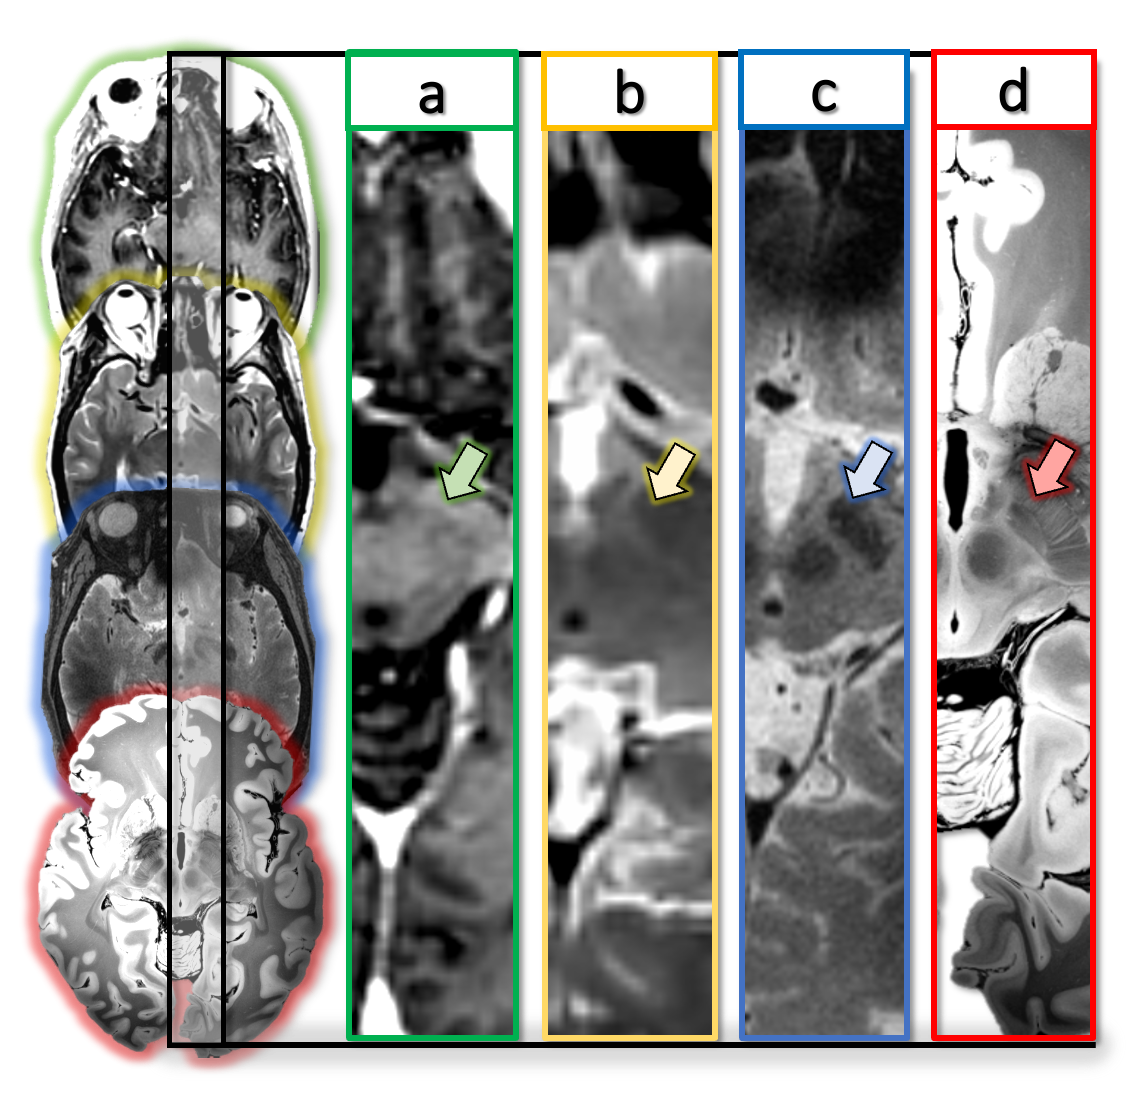
\includegraphics[width=1\linewidth]{figs/ch1_Figure_STN_MRI.png}
    \caption{
    Visualization of the subthalamic nucleus (STN) across different MRI modalities. (a) Clinically acquired T1-weighted MRI (MP2RAGE) at 1.5 Tesla with gadolinium contrast, enhancing visualization of blood vessels. (b) T2-weighted MRI acquired from the same subject and scanner as in (a). (c) High-resolution T2-weighted MRI (SPACE sequence) acquired at 7 Tesla. (d) \textit{ex vivo} MRI acquired at 7 Tesla for comparison \cite{Edlow2020-mo}. The STN is indicated by colour-mapped labels.}
    \label{fig:ch1_Figure_STN_MRI}
\end{figure}

\textbf{T1-weighted MRI (T1w):} T1-weighted sequences, such as Magnetization-Prepared RApid Gradient Echo (MPRAGE), provide a detailed anatomical overview with high gray-white matter contrast \cite{Brant-Zawadzki1992-nw} and define important landmarks like the anterior and posterior commissures (AC-PC line). However, at clinical field strengths (i.e., 1.5 or 3 Tesla (T)), conventional T1w imaging offers limited contrast between deep gray matter structures themselves. For instance, the STN is poorly distinguished on standard T1w images.

\textbf{T2-weighted and FLAIR MRI (T2w/FLAIR):} T2-weighted sequences highlight water content and offer improved contrast for visualizing deep brain structures. T2w images depict the STN as a hypointense (dark) almond-shaped region distinguishable from surrounding BG anatomy. T2-FLAIR (fluid-attenuated inversion recovery) sequences suppress cerebrospinal fluid signals and enhance contrast at tissue interfaces, facilitating delineation of boundaries within the thalamus and pallidum. While direct comparisons between FLAIR and other imaging modalities remain limited \cite{Boutet2021-vg}, a 3T FLAIR sequence employing sampling perfection with application-optimized contrasts by using different flip angle evolution (SPACE) for preoperative targeting resulted in reduced geometric distortion and improved contrast with surrounding anatomy. Notably, this approach was associated with superior clinical outcomes at 12-month follow-up compared to conventional T2w imaging \cite{Senova2016-bh}.

\textbf{Inversion-Recovery MRI (FGATIR):}  
Fast Gray Matter Acquisition T1 Inversion Recovery (FGATIR) is a specialized MRI sequence designed to improve the visualization of deep gray matter structures for DBS targeting. Unlike conventional T1w or T2w scans, FGATIR employs a full 180° inversion pulse with a short inversion time to selectively nullify white matter signal, thereby enhancing contrast at the interface between gray and white matter. This feature is particularly useful in DBS planning, as many targets are embedded within heavily myelinated fiber tracts. A pilot study demonstrated that FGATIR provided clearer visualization of structures such as the internal medullary lamina of the GPi, the STN/substantia nigra interface, and fiber bundles from the internal capsule piercing the striatum-features not consistently resolved on other sequences \cite{Sudhyadhom2009-xx}. Quantitatively, FGATIR produced higher contrast-to-noise ratios (CNRs) across multiple regions of interest. For example, the CNR at the STN and substantia nigra was more than threefold higher on FGATIR compared to T2-FLAIR, facilitating better localization of the STN's inferior boundary. Overall, FGATIR offers a promising balance between contrast, resolution, and acquisition time for DBS planning, and has been increasingly adopted as a core component of multimodal MRI protocols for subcortical targeting \cite{Neudorfer2022-nj}.


\textbf{Susceptibility-Weighted Imaging and Quantitative Susceptibility Mapping (QSM):} MRI sequences sensitive to magnetic susceptibility-including T2*-weighted imaging, phase imaging, and QSM-exploit the iron content of deep brain nuclei. Structures like the STN are iron-rich and produce local magnetic field inhomogeneities detectable by these techniques. QSM, in particular, generates quantitative maps of magnetic susceptibility and provides superior contrast-to-noise ratios compared to conventional T2*-weighted imaging. This improved depiction facilitates more reliable boundary identification of small targets like the STN \cite{Liu2013-zm}, substantia nigra \cite{Chen2021-tj}, and zona incerta (ZI) \cite{Lau2020-dh} . Although susceptibility imaging is prone to artifacts-such as blooming distortions near air-tissue interfaces-QSM algorithms mitigate these effects by deconvolving the field perturbations, yielding more accurate anatomical localization.

\textbf{Diffusion-Weighted Imaging (DWI) and Tractography:} While conventional MRI depicts structural anatomy, diffusion MRI captures information about white matter pathways. Diffusion Tensor Imaging (DTI) and tractography methods can reconstruct fiber tracts that emanate from or pass near DBS targets \cite{Rodrigues2018-jt}. In clinical practice, tractography has supported a shift toward connectomic targeting, where stimulation is guided not solely by anatomy but also by network connectivity \cite{Horn2020-wf}. For example, tractography enables visualization of the corticospinal tract to avoid during Vim targeting for tremor, or the motor versus limbic subdivisions of the STN for tailored therapy \cite{Calabrese2016-xi}. Although DTI-based tractography lacks direct histological validation and is sensitive to distortions, it remains the only non-invasive method to visualize patient-specific brain networks \cite{Coenen2016-pd}, and is increasingly incorporated into DBS planning to optimize both therapeutic efficacy and side effect profiles.

By integrating these complementary MRI modalities, modern DBS planning protocols enhance the visualization of deep brain structures and fiber pathways. Although most DBS workflows use T1w imaging for stereotactic referencing (e.g., AC-PC annotation), all the other modalities are seldom used concurrently. Instead, DBS centers acquire one or two additional modalities depending on the target. This multimodal synergy reduced the reliance on indirect atlas-based approximations and exploratory microelectrode recordings. As a result, MRI-guided DBS has improved targeting precision, reduced operative times, and expanded the scope of treatable disorders through anatomically and network-informed strategies.

\subsection{Ultra-High Field MRI}
\label{sec:uhf_mri_physics}

Ultra-high field (UHF) MRI, defined as systems operating at magnetic field strengths of 7T or higher, offers significant advantages in neuroimaging due to fundamental physical improvements in signal acquisition. These gains directly translate into enhanced visualization of deep brain structures relevant to DBS targeting.

The signal-to-noise ratio (SNR) in MRI increases approximately linearly with magnetic field strength, with 7T MRI offering a 2--3-fold improvement over 3T systems \cite{Trampel2019-fa}. This gain in SNR can be traded for higher spatial resolution, which is particularly advantageous for DBS planning. For example, 7T MRI enables the acquisition of isotropic voxels as small as 0.5~mm, improving the delineation of small deep brain structures and their subregions. This benefit can be illustrated using the STN, a common DBS target with an estimated volume of 240~mm\textsuperscript{3} and a maximal extent of approximately 10~mm. At standard clinical resolution (1~mm isotropic), the STN is represented by roughly 240 voxels, with only 10 voxels spanning its longest axis. Each voxel encompasses an estimated 2300--2400 neurons \cite{Hamani2004-zr,Hardman2002-ru}, reducing anatomical specificity. Increasing spatial resolution to 0.5~mm isotropic increases the total voxel count to approximately 1920, with about 20 voxels along the nucleus’s longest dimension. At this finer scale, each voxel represents around 300 neurons, significantly enhancing anatomical fidelity and reducing partial volume effects.

Tissue relaxation properties undergo significant changes that enhance MRI contrast between different brain structures at 7T. Specifically, T1 relaxation times increase, and T2* relaxation times decrease, leading to improved differentiation between gray and white matter. This enhanced contrast is particularly beneficial for visualizing small and previously elusive deep brain nuclei, which are critical targets in DBS procedures. One notable example is the zona incerta (ZI), a small gray matter region situated in the subthalamic area. Historically, the ZI has been challenging to visualize in vivo due to its size and location. However, recent advancements have demonstrated that high-resolution T1 mapping at 7T allows for robust visualization of the ZI and its surrounding white matter structures along the entire rostrocaudal axis. This capability enables comprehensive anatomical characterization of this previously obscure deep brain region, facilitating more accurate DBS targeting \cite{Lau2020-dh}. Similarly, the delineation of intra-thalamic nuclei has been significantly improved at 7T. By adjusting inversion times to null white matter signals, enhanced contrast between thalamic nuclei can enable their reliable identification and segmentation. This advancement holds promise for refining DBS targeting strategies, particularly for conditions like essential tremor, where DBS is targeting specific thalamic nuclei \cite{Tourdias2014-un}.

Moreover, as shown in a comparative imaging study by Forstmann and colleagues, even when 3T images are highly optimized, they fail to match the clarity, boundary sharpness, and contrast seen in 7T acquisitions. For example, the STN and globus pallidus demonstrate significantly sharper lateral and posterior borders at 7T under T2*-weighted protocols. Additionally, the ventral intermediate nucleus (VIM) of the thalamus-difficult to delineate directly at any field strength-becomes more reliably identified through the improved contrast of neighboring thalamic nuclei at 7T \cite{Forstmann2017-gz}. Furthermore, a comparative outcome study by Middlebrooks and colleagues directly assessed patients undergoing DBS for essential tremor planned using either 3T or 7T MRI. Patients in the 7T cohort experienced significantly greater tremor reduction and required lower stimulation currents. Although the average electrode positions were comparable, the 7T cohort demonstrated significantly lower variance in the final location of the electrode, underscoring higher targeting precision during DBS \cite{Middlebrooks2024-gb}.

UHF MRI has advanced the visualization of deep brain structures, offering unprecedented contrast and resolution that enhance DBS targeting \cite{Isaacs2020-gq}. However, its integration into clinical workflows remains limited by both technical and logistical constraints. First, susceptibility artifacts-exacerbated at air-tissue interfaces near the skull base-can impair signal fidelity in regions adjacent to common DBS targets. Second, increased \(B_0\) and \(B_1\) field inhomogeneities at 7T introduce signal dropouts and nonuniform contrast, complicating the interpretation of small, deep nuclei \cite{Okada2022-fg}. Additionally, the higher specific absorption rate (SAR) at ultra-high field strengths may restrict sequence design and limit the use of certain clinically useful protocols, such as long echo-train or spin-echo–based acquisitions \cite{Okada2022-ln}. Spatial distortions-driven by both system-related nonlinearity and patient-specific susceptibility effects-can result in displacements of up to 2 mm near midbrain targets \cite{Kirby2023-la}, and distortion correction algorithms may introduce secondary errors if improperly applied. Beyond these imaging-specific limitations, widespread clinical adoption is also hindered by the limited availability of 7T systems globally, as they remain concentrated in research centers and require specialized infrastructure, coils, and workflows \cite{Forstmann2017-gz,Boutet2021-vg}. These challenges underscore a need for hybrid imaging and prepossessing strategies, alongside workflow standardization during DBS.

\subsection{Limitations of MRI in DBS Targeting}
\label{sec:MRI_limitations}

Despite significant advancements in MRI technology, several critical limitations hinder its optimal application in stereotactic planning for DBS. These challenges can be broadly categorized into issues related to sequence validation, anatomical generalizability, geometric fidelity, and clinical implementation.

\textbf{Lack of Standardization and Outcome-Linked Validation:} There is limited consensus on the most appropriate MRI sequences to directly visualize common DBS targets \cite{Vitek2010-cn,Middlebrooks2020-vv}. Although specialized sequences such as FGATIR and QSM have demonstrated improved visualization, few studies have rigorously compared these sequences or established their superiority in improving clinical outcomes compared to traditional indirect targeting methods \cite{Boutet2021-vg}. The lack of prospective validation and a unified protocol for DBS targeting remains a major gap in the literature.

\textbf{Limited Generalizability to Clinical Populations:}
Many MRI optimization studies have been conducted in healthy volunteers rather than the patient populations typically considered for DBS \cite{Boutet2021-vg}. These patients often exhibit disease-related and age-related brain atrophy, including reduced white matter volume \cite{Bonneville2005-vl,Lee2011-rf}, which can significantly affect the visibility of deep brain structures. As a result, sequences validated in healthy cohorts may underperform in clinical settings.

\textbf{Geometric Distortion and Registration Error:}
High-resolution MRI sequences-especially those using gradient-echo-based mechanisms (e.g., SWI, QSM)-are prone to geometric distortions arising from magnetic susceptibility effects. These distortions can compromise the spatial fidelity required for stereotactic neurosurgery, where errors of 1--2~mm can have significant clinical consequences \cite{Boutet2021-vg, Rasouli2018-sn, Lau2018-fp}. Furthermore, quantitative sequences (e.g., QSM) optimized for target visualization often fail to adequately depict anatomical landmarks or fiducials used in surgical navigation (e.g., AC and PC), necessitating registration to anatomical MRI or CT dataset. The accuracy of such registration pipelines is poorly quantified, and errors introduced in this step may accumulate and degrade targeting accuracy.

\textbf{Practical Constraints and Hardware Incompatibility:}
The implementation of advanced MRI sequences is often constrained by hardware limitations. For example, head coils that offer superior signal-to-noise ratios may not physically accommodate stereotactic head frames used in surgical planning \cite{Boutet2021-vg}. Similarly, while UHF MRI provides enhanced spatial resolution and contrast, it is currently incompatible with most commercial stereotactic systems and requires additional processing. Consequently, UHF images must be coregistered with stereotactic imaging from another modality (e.g., CT), a step that may introduce additional errors \cite{Lenglet2012-ii}.

\textbf{Experimental Status of Connectomic Techniques:}
Emerging techniques such as functional MRI and DWI tractography are beginning to reshape DBS targeting strategies by shifting focus from discrete anatomical nuclei to distributed structural and functional networks. Although retrospective studies suggest that connectomic targeting correlates with clinical response, these techniques remain largely experimental. Their clinical adoption is limited by a lack of prospective validation and the complexity of postprocessing pipelines \cite{Horn2017-bi}.

Thus, while MRI has greatly enhanced DBS targeting, it does not fully eliminate the need for complementary strategies such as multimodal imaging, atlas integration, and image registration pipelines to achieve the precision required for optimal outcomes. These solutions are further explored in the sections that follow.

\section{Image Registration}
\label{sec:registration}
Image registration is a fundamental step in neuroimaging analysis, facilitating spatial alignment of imaging volumes over time and modalities (e.g., MRI and CT) or to stereotactic spaces such as the MNI space \cite{Risholm2011-rm}. In DBS, registration plays a critical role in maintaining spatial continuity throughout the surgical workflow \cite{Geevarghese2016-qo}. Accurate coregistration ensures that anatomical information derived from preoperative MRI can be reliably transferred to stereotactic planning coordinates and subsequently reconciled with postoperative imaging for reliable DBS electrode localization and verification \cite{Lofredi2022-wi,Abbass2025-el}.

\subsection{Image Registration Fundamentals}
In its most general form, image registration aims to estimate a transformation \( v: \Omega_T \rightarrow \Omega_S \) that maps coordinates from the fixed image domain \( \Omega_T \) to the moving image domain \( \Omega_S \), such that the transformed moving image \( \tilde{S}(x) = S(v(x)) \) becomes aligned with the fixed image \( T(x) \). This process is commonly formulated as the following optimization problem:
\begin{equation}
    \arg\min_{v} \, \mathcal{C}(S \circ v, T) + \lambda \, \mathcal{R}(v)
    \label{eq:registration_loss}
\end{equation}

where \( \mathcal{C}(S \circ v, T) \) is a similarity metric that quantifies the alignment between the transformed moving image and the fixed image, \( \mathcal{R}(v) \) is a regularization term that encourages smoothness or anatomical plausibility of the transformation, and \( \lambda \) is a weighting parameter that balances data fidelity with regularization.

\paragraph{Transformation Models.}
Registration transformations are typically categorized based on their degrees of freedom (DoF), which determine how flexibly one image can be mapped to another \cite{Chen2023-wx, Zitova2003-ds, Maintz1998-gs}.

\begin{itemize}
    \item \textbf{Rigid} transformations preserve distances and angles by allowing only translation and rotation (6 DoF).
    
    \item \textbf{Affine} transformations extend rigid transformations by incorporating scaling and shearing (12 DoF), enabling global shape changes while preserving collinearity and parallelism.
\end{itemize}

Both rigid and affine transformations can be expressed in matrix form as:
\begin{equation}
    v(x) = \mathbf{M}x + t
    \label{eq:affine}
\end{equation}
where \( \mathbf{M} \in \mathbb{R}^{3 \times 3} \) encodes linear transformations (rotation, scaling, shear), and \( t \in \mathbb{R}^3 \) is a translation vector. 

These transformation models are computationally efficient and commonly used for intra-subject alignment across imaging sessions or modalities, where the underlying anatomy remains relatively unchanged \cite{Jenkinson2002-ab}. However, their global nature limits their ability to capture localized anatomical differences, which is particularly important in populations with neurodegeneration, lesions, tumors, or developmental abnormalities. Consequently, rigid and affine transformations are frequently employed as initialization steps for more flexible, nonlinear registration approaches.
\begin{itemize}
\item \textbf{Nonlinear (Deformable)} transformations introduce spatially varying displacements to capture local anatomical variation:
\begin{equation}
    v(x) = x + u(x)
    \label{eq:deformable}
\end{equation}
\end{itemize}
where \( u(x) \) is a dense smooth displacement field defined in the image domain. 

These transformations can accommodate complex inter-subject differences and are essential for high-precision applications such as brain morphometry, longitudinal studies, and label propagation from atlases. The most commonly used implementation diffeomorphic frameworks such as Symmetric Normalization (SyN) \cite{Avants2008-ek, Beg2005-yo}.

\paragraph{Similarity Metrics.}
To quantify alignment quality between the fixed image \( T(x) \) and the transformed moving image \( \tilde{S}(x) \), similarity metrics assess how well image intensities correspond after transformation. The choice of metric depends on the imaging modality and underlying intensity relationships:

\begin{itemize}
    \item \textbf{Sum of Squared Differences (SSD)} is a simple intensity-based metric suitable for \textit{intra-modality} registration, where images share similar intensity profiles. It assumes a linear relationship between corresponding intensities and penalizes squared voxel-wise differences:
    \begin{equation}
        \mathcal{C}_{\text{SSD}}(T, \tilde{S}) = \sum_{x \in \Omega_T} \left( T(x) - \tilde{S}(x) \right)^2
        \label{eq:ssd}
    \end{equation}
    SSD is computationally efficient but sensitive to noise and intensity non-uniformities~\cite{Zitova2003-ds,Maintz1998-gs}.

    \item \textbf{Normalized Cross-Correlation (NCC)} compares local intensity patterns and compensates for global intensity shifts or scaling. It is defined as:
    \begin{equation}
        \mathcal{C}_{\text{NCC}}(T, \tilde{S}) = \frac{\sum_x (T(x) - \mu_T)(\tilde{S}(x) - \mu_{\tilde{S}})}{\|T - \mu_T\| \cdot \|\tilde{S} - \mu_{\tilde{S}}\|}
        \label{eq:ncc}
    \end{equation}
    where \( \mu_T \) and \( \mu_{\tilde{S}} \) are the mean intensities of the fixed and moving images, respectively. NCC is robust to linear intensity variations and is often used in rigid and affine intra-modality registration~\cite{Pluim2003-kb}.

    \item \textbf{Mutual Information (MI)} measures the statistical dependence between intensity values in multimodal images. It is defined as:
    \begin{equation}
        \mathcal{C}_{\text{MI}}(T, \tilde{S}) = - \left[ H(T) + H(\tilde{S}) - H(T, \tilde{S}) \right]
        \label{eq:mi}
    \end{equation}
    where \( H(\cdot) \) denotes Shannon entropy and \( H(T, \tilde{S}) \) is the joint entropy. MI is robust to modality differences and widely used in scenarios like MRI--CT registration~\cite{Maes1997-jb,Wells1996-at}.
\end{itemize}

\paragraph{Optimization and Regularization.}
Optimization strategies include multiresolution gradient descent, Powell methods, or stochastic algorithms, and are chosen based on the complexity of transformations and the metric used \cite{Song2017-kq}. Regularization terms \( \mathcal{R}(v) \) ensure that transformations are smooth and physically meaningful, especially in deformable registration, where large local variations could lead to anatomically implausible deformation warps \cite{Castano-Aguirre2024-db}.

\subsection{Brain Templates and Atlases}
\label{sec:template_atlas}
Early stereotactic neurosurgical procedures were guided by knowledge from cadaveric specimens and sections. Atlases such as those by Talairach and Tournoux \cite{Talairach1957-eb,Talairach1988-wk} or Schaltenbrand-Wahren \cite{Schaltenbrand1977-ge} provided sectional views of the brain with overlaid coordinate systems anchored to internal features like the AC and PC line. These atlases were designed to support proportional scaling, allowing neurosurgeons to infer the location of deep brain structures relative to patient anatomy using intraoperative imaging modalities such as ventriculography or angiography \cite{Conti2023-oo}. Through these frameworks, atlas-based targeting became a central feature of stereotactic planning.

The advent of digital neuroimaging transformed atlas-based targeting. With the introduction of MRI and CT, and later population-averaged anatomical datasets, the field shifted from fixed, printed atlases toward deformable, individualized imaging. This shift introduced a useful conceptual distinction: a \textbf{template} is now understood as a coordinate-defined brain volume-often an average of many individuals-that serves as a registration target for aligning individual images. Examples include the MNI templates \cite{Avants2008-ek,Fonov2009-oi}, which define modern stereotactic spaces.

An \textbf{atlas}, by contrast, is now commonly defined as an annotation or labeling schema superimposed onto a template \cite{Chakravarty2006-ln}. These can include deterministic labels (e.g., segmentations of the STN) or probabilistic maps reflecting anatomical variability. An example is the DBS Intrinsic Template AtLas (DISTAL), which is a subcortical atlas based on a multimodal, high definition MNI template series, histology and tractography \cite{Ewert2018-bn}. In practice, a subject's MRI is first registered to a template via nonlinear transformation; only then can atlas labels be transferred and interpreted in the subject's anatomical context.

Stereotactic spaces serve as common reference systems for aligning brain images, enabling comparisons between subjects and large-scale studies. This spatial standardization supported automated meta-analytic tools such as \texttt{NeuroSynth} \cite{Yarkoni2011-sr} and \texttt{NeuroQuery} \cite{Dockes2020-nw}, which aggregated reported coordinates from thousands of studies to identify consistent associations between brain and behavior. Stereotactic spaces allowed the neuroimaging community to build reproducible and interpretable models of the brain structure and function at the population level.

In DBS, stereotactic spaces serve two main goals: 1) during target localization and planning to visualize conspicuous targets \cite{Stancanello2006-vj} and 2) registration to a population-based template is employed by the majority of studies that attempt to understand stimulation effects on targeted neural circuits \cite{Neudorfer2023-wd}.

\subsection{Registration Tools and Pipelines}
Classical registration algorithms rely on similarity metrics (e.g., NCC or MI) and optimization strategies to estimate transformations that align a moving image to a fixed reference \cite{Hoffmann2024-yd}. Tools such as FMRIB's Linear Image Registration Tool (\texttt{FLIRT}) provide robust linear registration through affine transforms of six or twelve dof \cite{Jenkinson2001-bw, Jenkinson2002-ab}. However, to capture anatomical variability between individuals, nonlinear registration is typically required \cite{Klein2009-lv}. Tools such as FMRIB's Non-Linear Image Registration Tool (\texttt{FNIRT}; \cite{Jenkinson2001-bw}), Advanced Normalization Tools (\texttt{ANTs}; \cite{Avants2011-zs}) and Statistical Parametric Mapping (\texttt{SPM}; \cite{Ashburner2007-en}) implement deformable models that estimate dense and smooth displacement fields across the brain.

Comparative studies \cite{Klein2009-lv, Ewert2019-cc} previously evaluated the performance of various nonlinear deformation algorithms across more than 45,000 registrations. Their findings revealed that tools like \texttt{ANTs}, and SPM's Diffeomorphic Anatomical Registration using Exponentiated Lie algebra (DARTEL) consistently ranked highest in accuracy across multiple datasets and labeling protocols, underscoring their reliability in gross morphological alignment tasks.

Recent advances in deep learning (see Section~\ref{sec:deeplearning}) have introduced registration frameworks like \texttt{SynthMorph} \cite{Hoffmann2024-yd} and \texttt{EasyReg} \cite{Iglesias2023-ni}, which offer fast, anatomy-aware, and acquisition-agnostic affine and deformable registration. Both of \texttt{SynthMorph} and \texttt{EasyReg} are trained on synthetic data generated from label maps, enabling robust generalization across contrasts and resolutions. Unlike traditional methods that require manual tuning and preprocessing, deep learning driven registration performs joint affine-deformable registration without preprocessing, offering a reproducible, high-throughput alternative with state-of-the-art performance across diverse neuroimaging datasets. 

Modern preprocessing pipelines incorporate these tools into modular workflows. For instance, \texttt{fMRIPrep} is an analysis pipeline designed for robust anatomical and functional MRI preprocessing \cite{Esteban2019-oz}. It integrates tools from \texttt{ANTs}, \texttt{FreeSurfer} \cite{Fischl2012-dp}, \texttt{FSL}, and others to standardize preprocessing across diverse acquisition protocols while maximizing transparency via detailed quality reports. Although developed for functional MRI, its anatomical pipeline performs high-quality T1-to-template registration using \texttt{ANT's} symmetric diffeomorphic normalization (SyN) with careful bias correction and skull stripping. Similarly, \texttt{Lead-DBS} is a dedicated pipeline tailored for DBS imaging. It supports multispectral co-registration, subcortical-optimized normalization, and electrode reconstruction across clinical and research imaging environments. \texttt{Lead-DBS} incorporates nonlinear warping methods from \texttt{ANTs}, \texttt{SPM}, and \texttt{FSL}, and its registration performance has been evaluated across over 11,000 deformations for subcortical alignment. The validation paper \cite{Ewert2019-cc} demonstrated that multispectral normalization (e.g., using T1w and T2w images) improved the registration of DBS targets such as the STN and GPi to template space, yielding segmentation accuracies comparable to manual labels. 

In neurosurgical applications such as DBS, millimetric registration accuracy is critical. Thus, pipelines like \texttt{Lead-DBS} emphasize subcortical-focused normalization and brain-shift correction, and allow for visual inspection of co-registrations and electrode reconstructions \cite{Neudorfer2023-wd}. The increasing integration of registration pipelines with atlases and connectivity models has further enhanced their utility in DBS targeting, enabling patient-specific analyses anchored to standardized anatomical references.

\subsection{Limitations in Validation and Quality Control}
Despite its importance, image registration remains a major source of spatial error in neuroimaging pipelines \cite{Lau2019-eh, Abbass2022-lf}. The accuracy of registration can be influenced by various factors, including voxel size, contrast properties, presence of artifacts, and the choice of template or deformation model \cite{Klein2009-lv, Ewert2019-cc}. Yet, in practice, assessing the quality of a registration often depends on surrogate measures that may not always reflect true anatomical alignment.

Voxel overlap metrics such as the Dice or Jaccard coefficients remain widely used for evaluating registration performance. However, these measures are unitless and provide limited spatial quantification of alignment error. This lack of physical interpretability presents a significant limitation in neurosurgical contexts, where magnitude and directionality of spatial misalignment can impact clinical outcomes. Moreover, the dynamic range of voxel overlap metrics is relatively narrow—once a threshold of moderate overlap is achieved, these measures often saturate, making them insensitive to subtle but clinically meaningful misregistrations \cite{Lau2019-eh}. Beyond interpretability and dynamic range, the calculation of voxel overlap metrics requires accurate and reliable anatomical segmentations. Manual segmentation of brain structures is labor-intensive and requires expert anatomical knowledge. Automated segmentation methods, while efficient, may not always be trustworthy in cases of anatomical distortion, image noise, or low tissue contrast. These challenges collectively limit the utility of voxel overlap as a dependable measure for quality control in high-precision applications in neurosurgery.

Visual inspection remains the main mechanism for assessing registration quality in both research and clinical settings \cite{Neudorfer2023-wd,Esteban2019-oz}. However, this method is inherently subjective and may not reliably detect local or focal misregistrations, especially in deep brain regions with indistinct anatomical boundaries \cite{Bosma2024-cf,Rohlfing2012-kt}. Even experienced raters may overlook errors when differences are subtle or distributed across non-obvious regions of the image \cite{de-Senneville2020-am}. Furthermore, visual inspection of reformatted, subtraction, or variance images cannot always reliably distinguish accurate from inaccurate registrations \cite{Rohlfing2012-kt}. As a result, sole reliance on visual inspection risks underestimating the registration error, especially in an application like DBS where millimetric spatial correspondence is essential for optimal therapeutic benefit and minimizing side effects.

\section{Brain Coordinates} 
A fiducial, from 'fiducia' in Latin meaning trust or confidence, is a point of reference that marks a specific identifiable location in space. In neuroanatomy, a fiducial typically represents a reproducible anatomical feature, such as the AC or PC. These points serve as spatial anchors for assessing anatomical correspondence \cite{Schonecker2009-xj,Lau2019-eh} or describing and understanding the structure of the brain \cite{Abbass2022-lf}. The use of fiducials is rooted in classical stereotactic approaches, where the localization of deep brain structures depended on point-based references that were visible in imaging modalities or in postmortem atlases \cite{Schaltenbrand1977-ge, Talalrach1957-bs}. Fiducials are sometimes referred to as landmarks or markups \cite{Fedorov2012-rk}, although these terms are used interchangeably depending on the application domain. 
\subsection{Fiducials for Registration and Brain Mapping}
While contemporary neuroimaging pipelines may often rely on voxel-wise or segmentation-based representations to evaluate correspondence \cite{Chakravarty2008-mt,Hoffmann2024-yd}, these methods may obscure local misalignments \cite{Lau2019-eh} and lack interpretability \cite{Rohlfing2012-kt}. Fiducials, by contrast, offer a human-interpretable method to assess spatial alignment in millimeters based on direct measurement of a vector describing point-to-point correspondence. This approach has particular value in stereotactic neurosurgery and atlas construction, where millimetric precision is critical. Distance metrics computed between homologous fiducial points in different images can provide sensitive and intuitive measures of spatial discrepancy, offering complementary insight to conventional similarity metrics (Figure \ref{fig:ch1_Figure_afidsvsoverlap}).

However, the value of fiducials can extend beyond ascertaining spatial correspondence. As spatial abstractions of anatomy, coordinates offer a compact, interpretable, and modality-agnostic representation of brain structure. When derived from reproducible landmarks, coordinates can be used to characterize anatomical geometry, measure morphological variability, track spatial consistency between imaging sessions or pipelines, and general anatomy-aware quality control of images. This point-based framework provides a physically grounded alternative to dense voxel-based fields, with the added benefit of dimensional simplicity and intuitive error quantification.

\begin{figure}[hbt!]
    \centering
    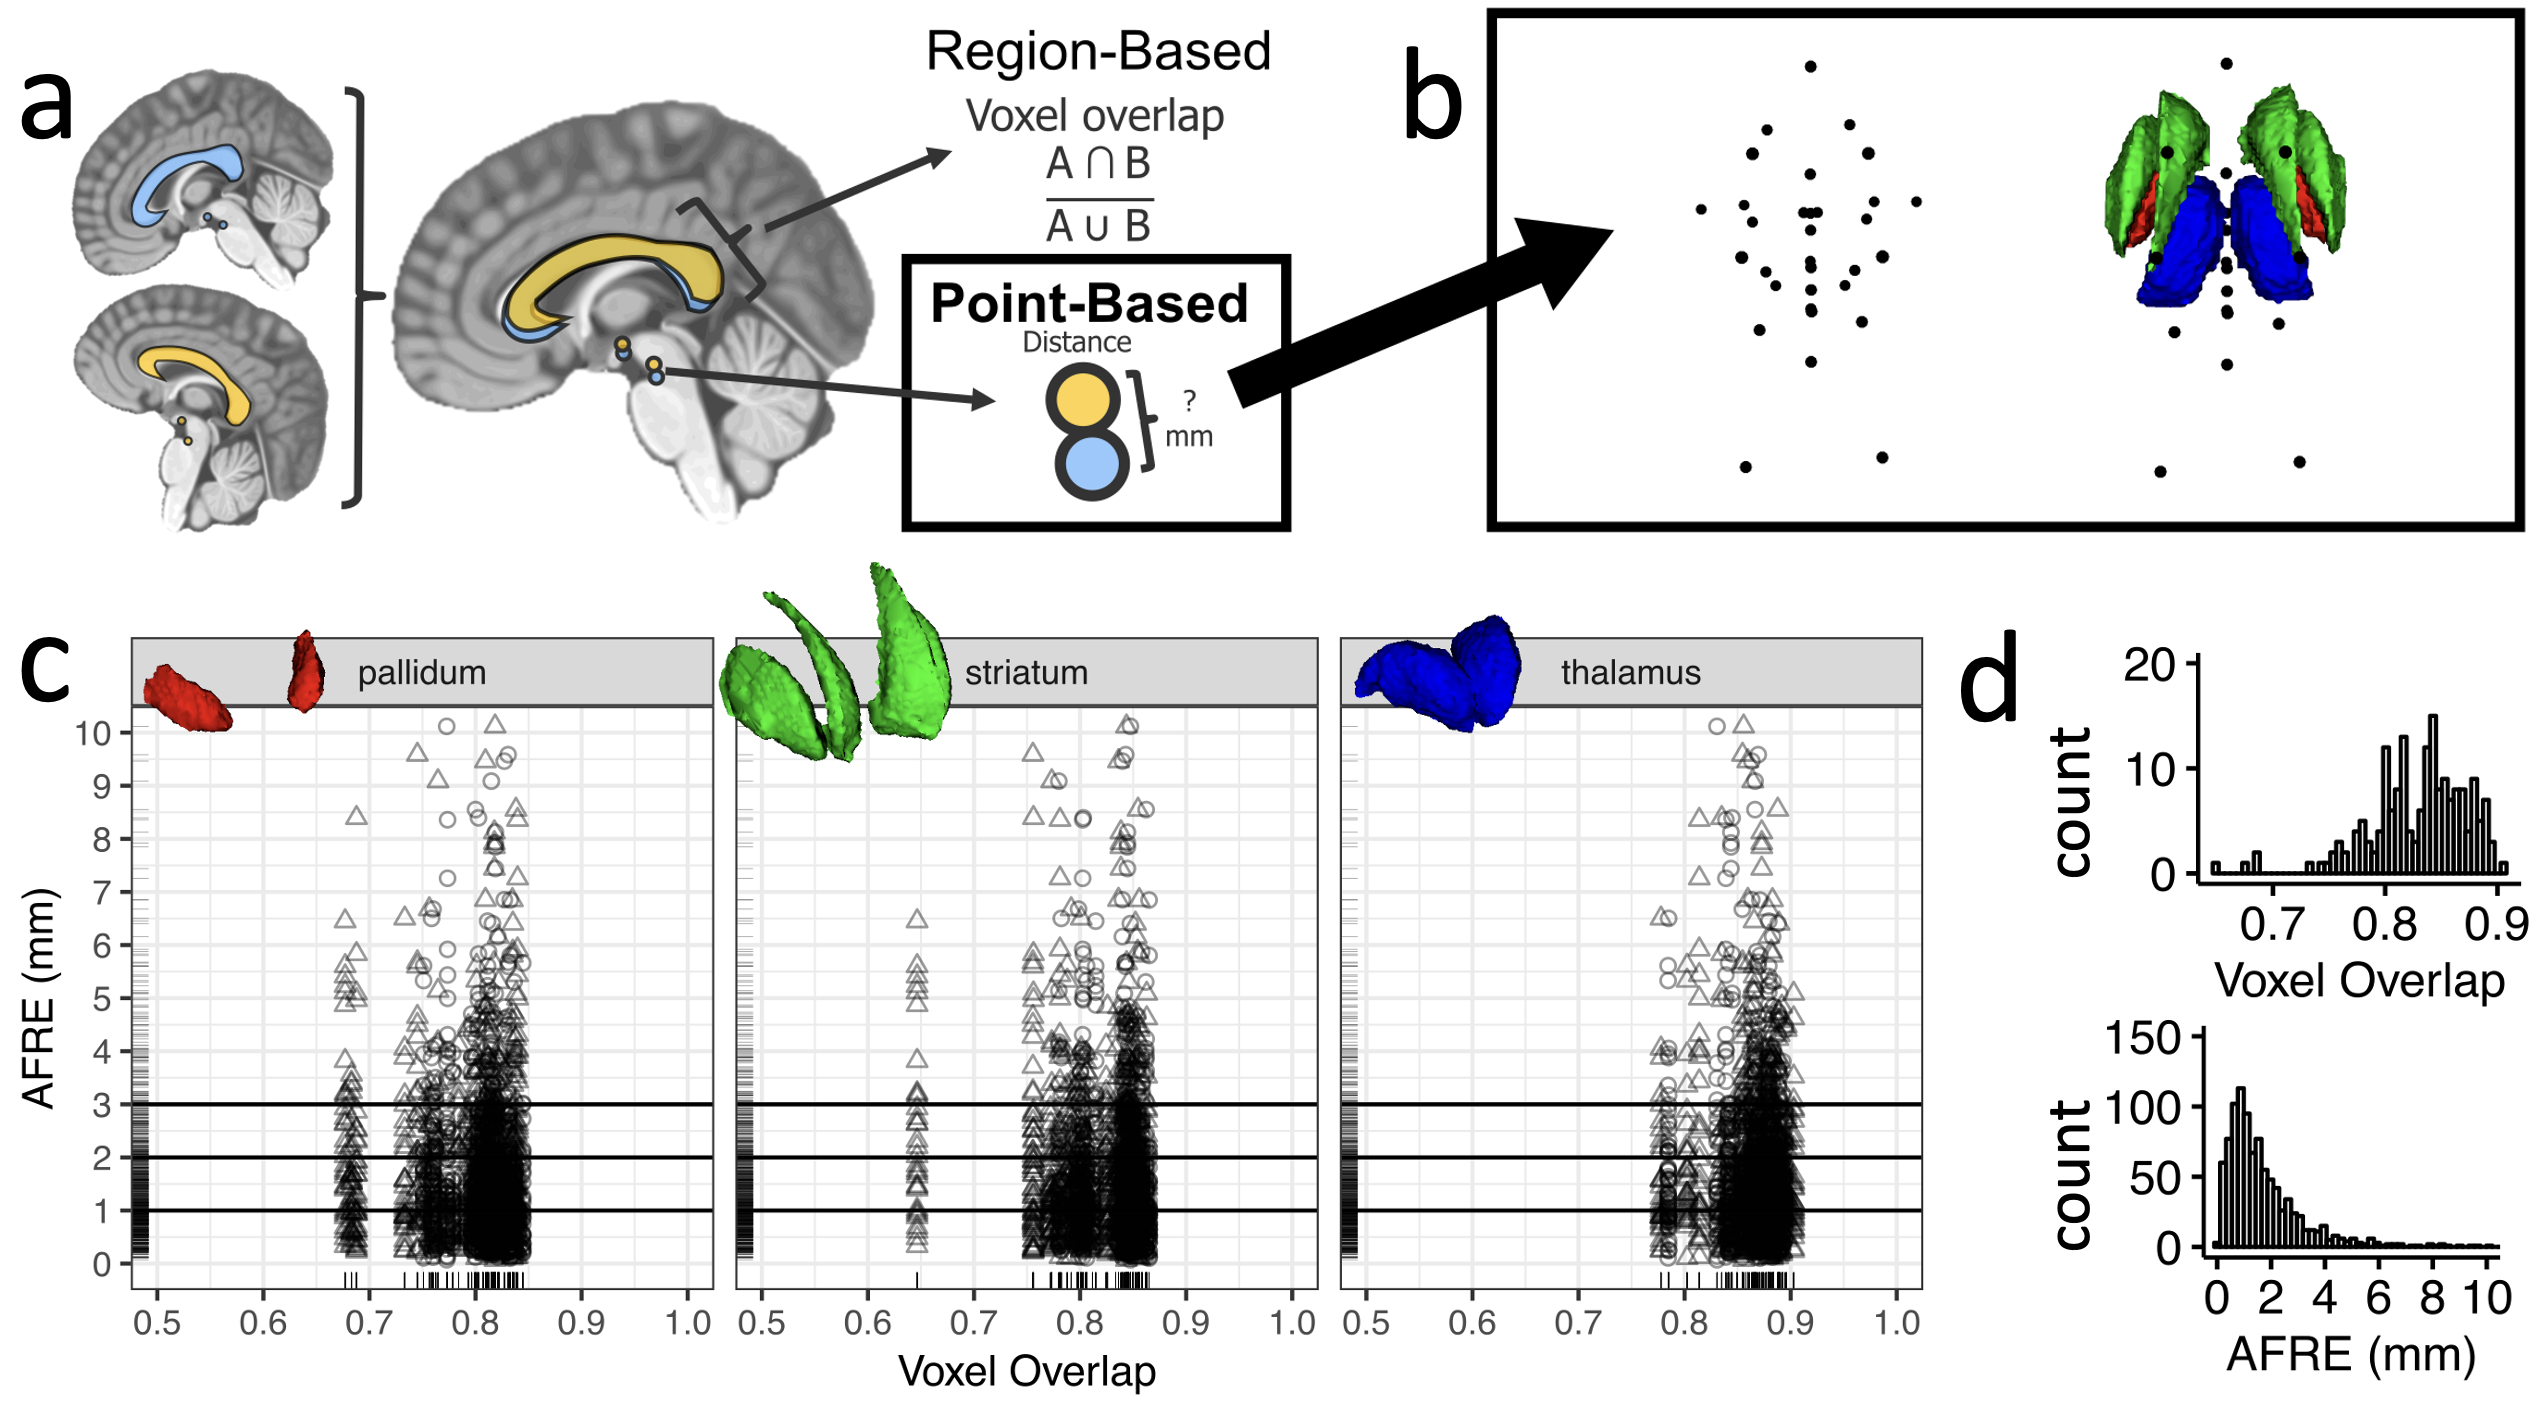
\includegraphics[width=1\linewidth]{figs/ch1_Figure_afidsvsoverlap2.png}
    \caption{Head-to-head comparison of region-based overlap metrics and point-based metrics for evaluating spatial correspondence. (a) Schematic illustrating the computation of registration error metrics using either voxel-wise overlap between homologous regions (i.e., voxel overlap) and points (i.e., anatomical fiducial registration error; AFRE). (b) Abstraction of the anatomical fiducials (AFIDs) framework, with fiducial points distributed across three regions: pallidum (red), striatum (green), and thalamus (blue). (c,d) Trellis plots comparing region-based and point-based metrics. AFRE demonstrates a more unimodal distribution and a clearer, millimeter-scale dynamic range relative to voxel overlap metrics. Figure modified from an open-access article by \cite{Lau2019-eh}}
    \label{fig:ch1_Figure_afidsvsoverlap}
\end{figure}

\subsection{The Anatomical Fiducials Framework}
The Anatomical Fiducials (AFID) protocol is an open-access reference for the placement of fiducials in MRI \cite{Lau2019-eh}. These fiducials are defined based on reproducible neuroanatomical landmarks that span ventricular, sulcal, commissural, and deep brain regions. The goal of the protocol is to enable consistent and interpretable mapping of brain anatomy across individuals, imaging modalities, and spatial references (Figure .

Fiducials are placed manually by trained raters following a detailed anatomical definition guide, which includes visual references and 3D renderings to support accurate localization. Each AFID corresponds to a specific anatomical feature and is associated with a single point in the subject's native image space. The placement process typically requires a standard T1-weighted MRI scans, which provides sufficient contrast for identifying the underlying structure.

The resulting set of AFID coordinates forms a sparse point cloud that captures the spatial configuration of various areas of the brain. This point cloud can be used for a variety of downstream applications, including quality control of image registration, benchmarking of automated segmentation algorithms, and geometric morphometric analysis. Because AFIDs are interpretable and grounded in clearly defined anatomy, they are particularly well suited for assessing spatial transformations, including those involving deformation fields.

The AFIDs protocol has been validated in healthy controls and patient populations on T1w MRI, demonstrating inter-rater reliability on the order of 1-2 millimeters. Furthermore, it builds on open-source software infrastructures that support training, visualization, and analysis. The AFIDs protocol can become a valuable resource for researchers and clinicians seeking to quantify spatial accuracy and ensure anatomical fidelity in neuroimaging workflows.

\section{Machine Learning}
The field of neuroimaging has been transformed by the convergence of two powerful trends: (1) the availability of large-scale imaging datasets and (2) advances in computational methods. Open access datasets such as the Human Connectome Project (HCP; \cite{Van_Essen2013-yi}), UK Biobank \cite{Sudlow2015-lq}, Alzheimer's Disease Neuroimaging Initiative (ADNI; \cite{Petersen2010-rd}, and Parkinson's Progression Markers Initiative (PPMI; \cite{Marek2018-wx}) facilitated large-scale studies of brain structure, function, and disease. At the same time, improvements in computational resources—particularly the widespread availability of graphics processing units (GPU), high-performance computing clusters (HPC), and cloud-based infrastructure—have enabled the efficient training and deployment of complex machine learning (ML) models on high-dimensional neuroimaging data, dramatically accelerating both research and clinical translation \cite{Bouchard2016-cd,Kirimtat2024-is}.

\subsection{Overview of Machine Learning}
ML constitutes a methodologically diverse subfield of artificial intelligence that encompasses statistical techniques for developing computational algorithms capable of iterative self-improvement through data exposure and performance feedback \cite{Sarker2021-ng}. These algorithms demonstrate the capacity to recognize complex patterns, establish multidimensional relationships, and generate predictions from high-dimensional data without explicit rule-based programming \cite{Davatzikos2019-zq}.

ML operates through four fundamental processes: (1) Data preparation transforms raw input into suitable representations, often involving feature selection and normalization  \cite{Mwangi2014-nl}. (2) Model training adjusts parameters to minimize prediction errors on labeled examples, using optimization methods to find the best-fitting solution \cite{Lemm2011-jm}. (3) Regularization techniques balance the trade-off between fitting training data and maintaining generalizability to new examples \cite{Roberts2021-ib}. (4) Model inference tests performance on unseen data to ensure generalization beyond training examples, using metrics appropriate to the specific task \cite{Varoquaux2022-as}.  These processes work in concert to create systems that can recognize patterns and make predictions with increasing accuracy as they process more data.

ML methodologies are characterized by distinct learning paradigms based on the training data available and ultimate objective of the ML model. These paradigms are generally supervised, unsupervised, semi-supervised and reinforcement learning \cite{Hastie2009-ef}. \textbf{Supervised learning} optimizes algorithms using labeled training data, where each input is paired with corresponding output annotations; the algorithm learns to predict these outputs by minimizing the difference between its predictions and ground-truth labels. \textbf{Unsupervised learning} extracts intrinsic patterns from unlabeled data through dimensionality reduction or clustering algorithms, revealing underlying structures without predefined categories. \textbf{Semi-supervised learning} leverages both labeled and unlabeled data, addressing situations where annotations are limited while preserving generalization capabilities. \textbf{Reinforcement learning} enables algorithms to learn optimal behaviors through environmental interaction and feedback signals, its applications in medical imaging are limited compared to other paradigms \cite{Zhou2021-au}. 

These learning paradigms found natural applications in neuroimaging analysis, where the complexity and dimensionality of the data align with ML's pattern recognition strengths \cite{Vieira2017-vr}. The transition from general ML applications to medical imaging was particularly motivated by three factors:  (1) Standardized nature of medical image acquisition that facilitates algorithmic processing  \cite{Li2020-dy}. (2) Presence of anatomical patterns that remain relatively consistent across patients despite individual variations \cite{Iglesias2023-co}. (3) Potential for ML to address the time-intensive nature of manual image analysis in clinical workflows \cite{Khalifa2024-dn}. In the following sections, we outline the foundations of various ML models leveraged in this dissertation. 

\subsection{Traditional Machine Learning Models}
Traditional ML approaches in neuroimaging typically rely on handcrafted quantitative summary measures extracted from preprocessed scans using domain expertise and predefined anatomical or functional templates \cite{Mwangi2014-nl}. Common examples include regional brain volumes derived from segmentation protocols (e.g., hippocampal volume in Alzheimer’s disease), cortical thickness measurements from surface reconstructions (e.g., via FreeSurfer), white matter integrity metrics from DWI (e.g., fractional anisotropy), and voxel-wise signal intensities from structural or functional scans \cite{Abraham2014-va, Coupe2019-pe}. These features reduce the dimensionality of raw imaging data and make it more tractable for classical algorithms. Once extracted, these features are input into supervised learning algorithms (e.g., linear regression or random forests) which aim to map imaging-derived features to clinical or anatomical outcomes \cite{Mateos-Perez2018-xb,Jollans2019-mv,Sarica2017-dz}.

Ridge regression \cite{Hoerl1970-so} is a regularized linear model that addresses multicollinearity and overfitting by introducing an $\ell_2$ penalty on the magnitude of the regression coefficients. Given a dataset with input features $\mathbf{X} \in \mathbb{R}^{n \times p}$ and target vector $\mathbf{y} \in \mathbb{R}^n$, ridge regression estimates the coefficient vector $\boldsymbol{\beta} \in \mathbb{R}^p$ by minimizing the following objective function:

\begin{equation}
    \mathcal{L}_{\text{ridge}}(\boldsymbol{\beta}) = \|\mathbf{y} - \mathbf{X}\boldsymbol{\beta}\|_2^2 + \lambda \|\boldsymbol{\beta}\|_2^2,
\end{equation}

where $\lambda \geq 0$ is a regularization parameter controlling the trade-off between data fidelity and model complexity. This formulation encourages small coefficients and yields a stable solution even in the presence of many correlated predictors—a common scenario in neuroimaging applications where the number of features may exceed the number of samples.

In contrast, Extreme Gradient Boosting (XGBoost; \cite{Chen2016-ew}) is a nonlinear ensemble method based on gradient boosting of decision trees. It constructs a series of regression trees $\{f_m\}_{m=1}^M$, where each successive tree $f_m$ is trained to minimize the residual error of the current model:

\begin{equation}
    \hat{y}_i^{(m)} = \hat{y}_i^{(m-1)} + f_m(\mathbf{x}_i),
\end{equation}

and the overall objective includes a regularization term to penalize model complexity:

\begin{equation}
    \mathcal{L}_{\text{xgb}} = \sum_{i=1}^n \ell(y_i, \hat{y}_i) + \sum_{m=1}^M \Omega(f_m),
\end{equation}

where $\ell$ is a differentiable loss function (e.g., squared loss or logistic loss), and $\Omega(f_m)$ penalizes tree complexity (e.g., number of leaves and leaf weights). XGBoost can capture intricate nonlinear relationships and interactions between features, making it well-suited for high-dimensional imaging data with subtle and distributed signal patterns.

Both ridge regression and XGBoost are attractive in neuroimaging contexts due to their balance of performance, regularization control, and interpretability \cite{Rokem2020-vj,Yi2023-ak}. However, the performance of these models remains highly dependent on the quality and relevance of the chosen features \cite{Mwangi2014-nl}. Handcrafted features may fail to capture distributed or hierarchical patterns in the data, and models like ridge regression, while robust, assume linear relationships between inputs and outputs. Even flexible models like XGBoost, despite their ability to model nonlinearity, are only as powerful as the input features allow.

These limitations underscore the fact that traditional ML approaches, while foundational, are constrained by their indirect use of image data, their limited spatial expressiveness, and their dependence on predefined representations \cite{Varoquaux2022-as,Mwangi2014-nl}. This motivated the adoption of deep learning techniques \cite{Sarker2021-fo}, which seek to learn hierarchical and spatially grounded representations directly from raw neuroimaging data.

\subsection{Deep Learning Models}
\label{sec:deeplearning}
Deep learning (DL), a subfield of machine learning, enables models to learn hierarchical feature representations directly from raw data, removing the need for manual feature engineering \cite{LeCun2015-da, Sarker2021-fo}. Unlike traditional ML approaches that rely on predefined descriptors, DL models use multilayered artificial neural networks (ANNs) to automatically extract and combine increasingly abstract information through learned transformations. These networks are loosely inspired by the structure of biological neurons. The input is represented as a vector in the first layer of "neurons" and propagates through multiple hidden layers. Each neuron applies an affine transformation to the previous layer’s output followed by a nonlinear activation function:
\begin{equation}
    \mathbf{h}^{(l)} = \sigma\left( \mathbf{W}^{(l)} \mathbf{h}^{(l-1)} + \mathbf{b}^{(l)} \right),
\end{equation}

where $\mathbf{h}^{(l)}$ is the activation of layer $l$, $\mathbf{W}^{(l)}$ is the weight matrix, $\mathbf{b}^{(l)}$ is a bias vector, and $\sigma$ is a nonlinear function carefully chosen depending on application (e.g., Rectified Linear units or ReLU; \cite{Agarap2018-vg}). During training, these parameters are iteratively updated to minimize a task-specific loss function, allowing the model to build higher-level abstractions from raw input.

While effective for low-dimensional structured data, standard ANNs become impractical and do not account for the spatial structure of high-dimensional inputs such as 3D neuroimaging volumes. For example, flattening a \(64 \times 64 \times 64\) voxel patch would yield a 262,144-dimensional input vector, forcing each neuron in the first layer to learn a separate weight for every voxel. This results in massive parameter counts and a high risk of overfitting, while also discarding the spatial relationships inherent to image data. Convolutional neural networks (CNNs) address these issues using weight sharing and local receptive fields to preserve spatial structure while significantly reducing the number of learnable parameters \cite{LeCun2015-da,Indolia2018-vu}.

A CNN layer applies a learnable kernel \( w \in \mathbb{R}^{k \times k \times k} \) across the input volume via discrete convolution, producing feature maps that encode local spatial relationships. The output of a convolutional layer is given by:

\begin{equation}
    h^{(l)}_k = \sigma\left( \sum_{i=1}^{C^{(l-1)}} w^{(l)}_{ik} * h^{(l-1)}_i + b^{(l)}_k \right),
\end{equation}

where $h^{(l)}_k$ denotes the \(k\)-th feature map at layer \(l\), $*$ denotes convolution, and \(\sigma\) is an activation function. Deeper layers encode increasingly abstract representations by combining low-level features such as edges and textures into complex anatomical or pathological patterns.

One of the most influential architectures in biomedical image analysis is the U-Net \cite{Ronneberger2015-xm}, which uses an encoder–decoder structure to balance semantic context with spatial precision (Figure \ref{fig:ch1_Figure_UNET}). The encoder applies convolution and downsampling layers to extract global features, while the decoder path upsamples these features to recover spatial resolution using transposed convolutions. Crucially, skip connections between corresponding encoder and decoder layers allow early high-resolution features to be directly reused—preserving fine-grained spatial information that might otherwise be lost through pooling. Formally, the decoder reconstructs a segmentation map $\hat{Y} \in \mathbb{R}^{H \times W \times K}$ from a compressed latent representation $Z$ by applying learned upsampling operators. The inclusion of skip connections between corresponding encoder and decoder levels allows the model to retain fine-grained spatial information that would otherwise be lost through pooling.

U-Nets are typically trained using voxel-wise loss functions such as cross-entropy or the Dice coefficient:

\begin{equation}
    \mathcal{L}_{\text{Dice}} = 1 - \frac{2 \sum_i p_i g_i}{\sum_i p_i + \sum_i g_i},
\end{equation}

where $p_i$ and $g_i$ represent predicted and ground truth labels for voxel $i$, respectively. Variants such as 3D U-Net \cite{Cicek2016-dz} and V-Net \cite{Milletari2016-ra} extend the architecture to volumetric data, and have become the standard for tasks such as skull stripping \cite{Hoopes2022-al} and segmentation \cite{Billot2023-tl, DeKraker2022-gj}. Contemporary improvements include the incorporation of residual blocks, attention modules, and multi-scale feature fusion to improve robustness in low-contrast or morphologically variable regions \cite{Oktay2018-rh}. 

\begin{figure}[hbt!]
     \centering
     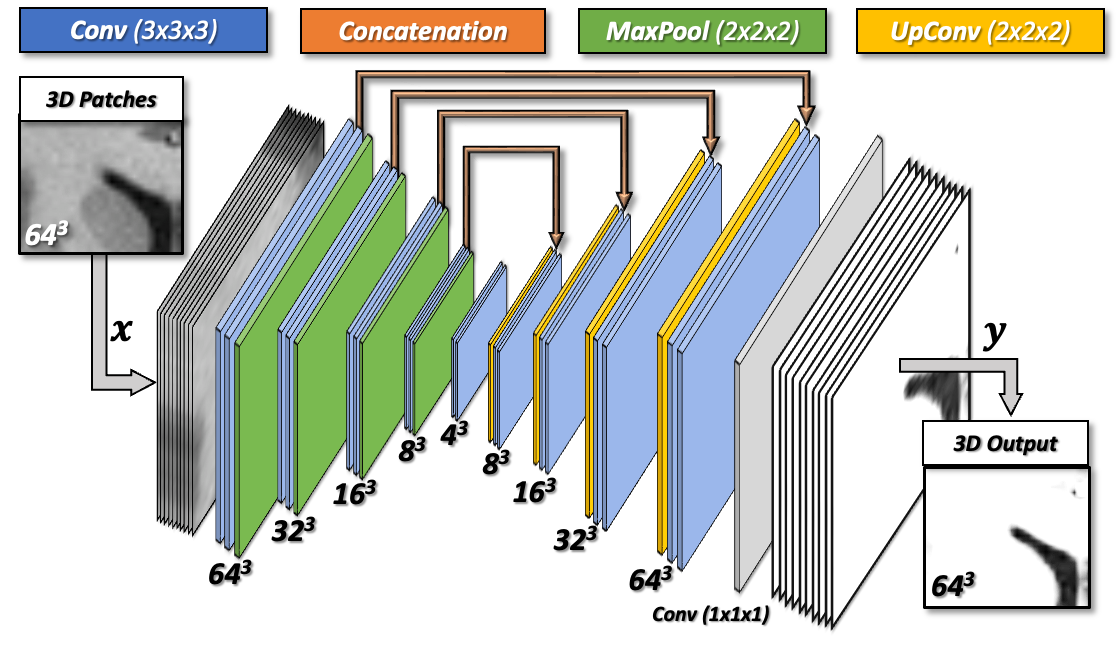
\includegraphics[width=1\linewidth]{figs/ch1_Figure_UNET.png}
     \caption{Schematic of an example 3D U-Net architecture \cite{Ronneberger2015-xm,Cicek2016-dz} used for volumetric image-to-image prediction. The input consists of $64^3$ voxel 3D patches, which undergo repeated convolution operations (blue; $3{\times}3{\times}3$ kernels) and spatial downsampling via max pooling (green; $2{\times}2{\times}2$). The encoder-decoder structure enables feature extraction at multiple scales, with skip connections (orange) preserving spatial information through concatenation. The decoder path applies upconvolutions (yellow; $2{\times}2{\times}2$) to restore resolution and generate the final $64^3$ voxel 3D output which depicts a brain ventricle segmentation as way of example.}
     \label{fig:ch1_Figure_UNET}
 \end{figure} 
 
Further advancements include nnU-Net \cite{Isensee2021-ev}, a self-configuring deep learning framework for biomedical image segmentation. Unlike traditional approaches that require manual tuning of preprocessing, network architecture, and training parameters, nnU-Net automates these decisions based on dataset-specific properties. Upon receiving a new dataset, nnU-Net analyzes its characteristics—such as image modality, size, and spacing—and configures a tailored segmentation pipeline. This includes selecting appropriate network architectures (e.g., 2D, 3D, or cascaded U-Nets), preprocessing steps, and post-processing techniques. This holistic approach has enabled nnU-Net to achieve state-of-the-art performance across 23 public datasets, surpassing many specialized methods with minimal manual intervention.

Although architectures such as U-Net were originally developed for image segmentation, they have also been adapted for point-based tasks such as anatomical landmark detection \cite{Ertl2025-wu,Chong2024-rp,Ye2023-wn}. Compared to segmentation, landmark detection in neuroimaging presents unique challenges: (1) Anatomical landmarks in brain MRI are often small and situated in regions of low contrast or homogeneous intensity. Many correspond to subtle anatomical features or geometric constructs, such as the midpoint of a structure or the intersection of internal axes, rather than distinct visual boundaries. Consequently, models must infer these points from contextual cues rather than relying on strong local image features. (2) Landmark detection involves predicting a highly localized signal against a vast background, leading to extreme class imbalance. Without careful loss function design or architectural modifications, models may converge to trivial solutions. These characteristics have motivated specialized network designs and training strategies that output spatial coordinates—either directly through coordinate regression heads \cite{Nibali2018-bu} or indirectly via heatmap prediction \cite{Payer2016-ik}.

\subsection{Challenges in Generalization and Interpretability}
Despite their promise, traditional ML and DL models face significant challenges in clinical neuroimaging. A major concern is generalization: models trained on data from a specific scanner, protocol, or population may not perform well when deployed in a different setting \cite{Davatzikos2019-zq}. Neuroimaging datasets are heterogeneous, where subtle differences in acquisition parameters can introduce bias. Efforts such as domain adaptation, harmonization, and transfer learning attempt to mitigate these effects, but the problem remains a barrier to clinical deployment \cite{Iglesias2023-co}. Furthermore, Many DL models function as "black boxes" that provide predictions without a clear explanation of their basis without explicit design \cite{Holzinger2019-kw}. This opacity can undermine clinician trust and complicate error analysis. Techniques such as saliency mapping, attention mechanisms, and feature attribution have been proposed to improve interpretability, but these methods may lack the spatial or clinical grounding necessary for anatomically meaningful insights \cite{Dinsdale2022-hf}.

\section{Open Science and Brain Imaging Data Structure}

Reproducibility and transparency are foundational to modern neuroimaging research, particularly as studies increasingly span large, heterogeneous datasets and complex analytical pipelines. The work in this dissertation embraces open science principles through the use of open data structures and code, version-controlled data management, and workflow automation tools that support reproducibility at scale.

\subsection{Brain Imaging Data Structure}

The Brain Imaging Data Structure (BIDS) \cite{Gorgolewski2016-oh} provides a standardized format for organizing and describing neuroimaging datasets. By specifying consistent directory hierarchies, file naming conventions, and metadata formats across imaging modalities, BIDS facilitates automated analysis, data sharing, and interoperability across tools. All imaging data used in this dissertation—including structural MRI volumes and anatomical fiducial annotations—are organized in BIDS-compliant formats and released openly. To manage datasets in a reproducible and decentralized manner, we adopt \texttt{datalad} \cite{Halchenko2021-px}, a data version control system that extends Git and Git-annex for large scientific datasets. \texttt{Datalad} enables efficient tracking of changes to imaging data, annotations, and model outputs across multiple machines and collaborators.

\subsection{Workflow Management}
As neuroimaging datasets grow in complexity and scale, reproducible and modular workflow management has become essential to ensure transparency and efficiency in data processing. Workflow engines provide a structured approach to defining and executing analytical pipelines, making it easier to track dependencies, scale computations, and share methods. In this work, we make use of \texttt{Snakemake} \cite{Molder2021-ig,Koster2012-ok}, a widely used workflow management system, together with \texttt{Snakebids} \cite{Van-Dyken-Tristan-Kuehn-Jason-Kai-Dahananjhay-Bansal-Ali-Khan2020-ay}, a companion interface that simplifies working with BIDS-organized neuroimaging data.

This BIDS-compliant framework provides a robust and extensible foundation for open, scalable, and reproducible neuroimaging research. By adhering to established standards and publicly releasing all data, code, and models, this dissertation contributes to the broader neuroimaging ecosystem—extending its utility to applications in stereotactic neurosurgery.

\section{Thesis Outline and Objectives}

This dissertation addresses the challenge of localizing brain structures with millimetric accuracy in a way that is scalable, interpretable, and clinically actionable. Deep brain stimulation surgery underscores the need to solve this challenge, where therapeutic targets such as the subthalamic nucleus are small, functionally heterogeneous, and situated within densely packed subcortical regions. Precise targeting is essential, yet the surgical planning process often relies on population-based maps generated through nonlinear image registration. These frameworks can introduce spatial errors on the same order as the targets themselves, complicating both individual treatment and broader scientific inference. At the same time, these same registration-based approaches are foundational to population neuroscience, where imaging data from many individuals is warped into a common stereotactic space to study brain structure, variability, and disease. In both settings—clinical and research—spatial uncertainty undermines confidence in localization and limits the translation of group-level findings to individual patients.

\begin{figure}[hbt!]
    \centering
    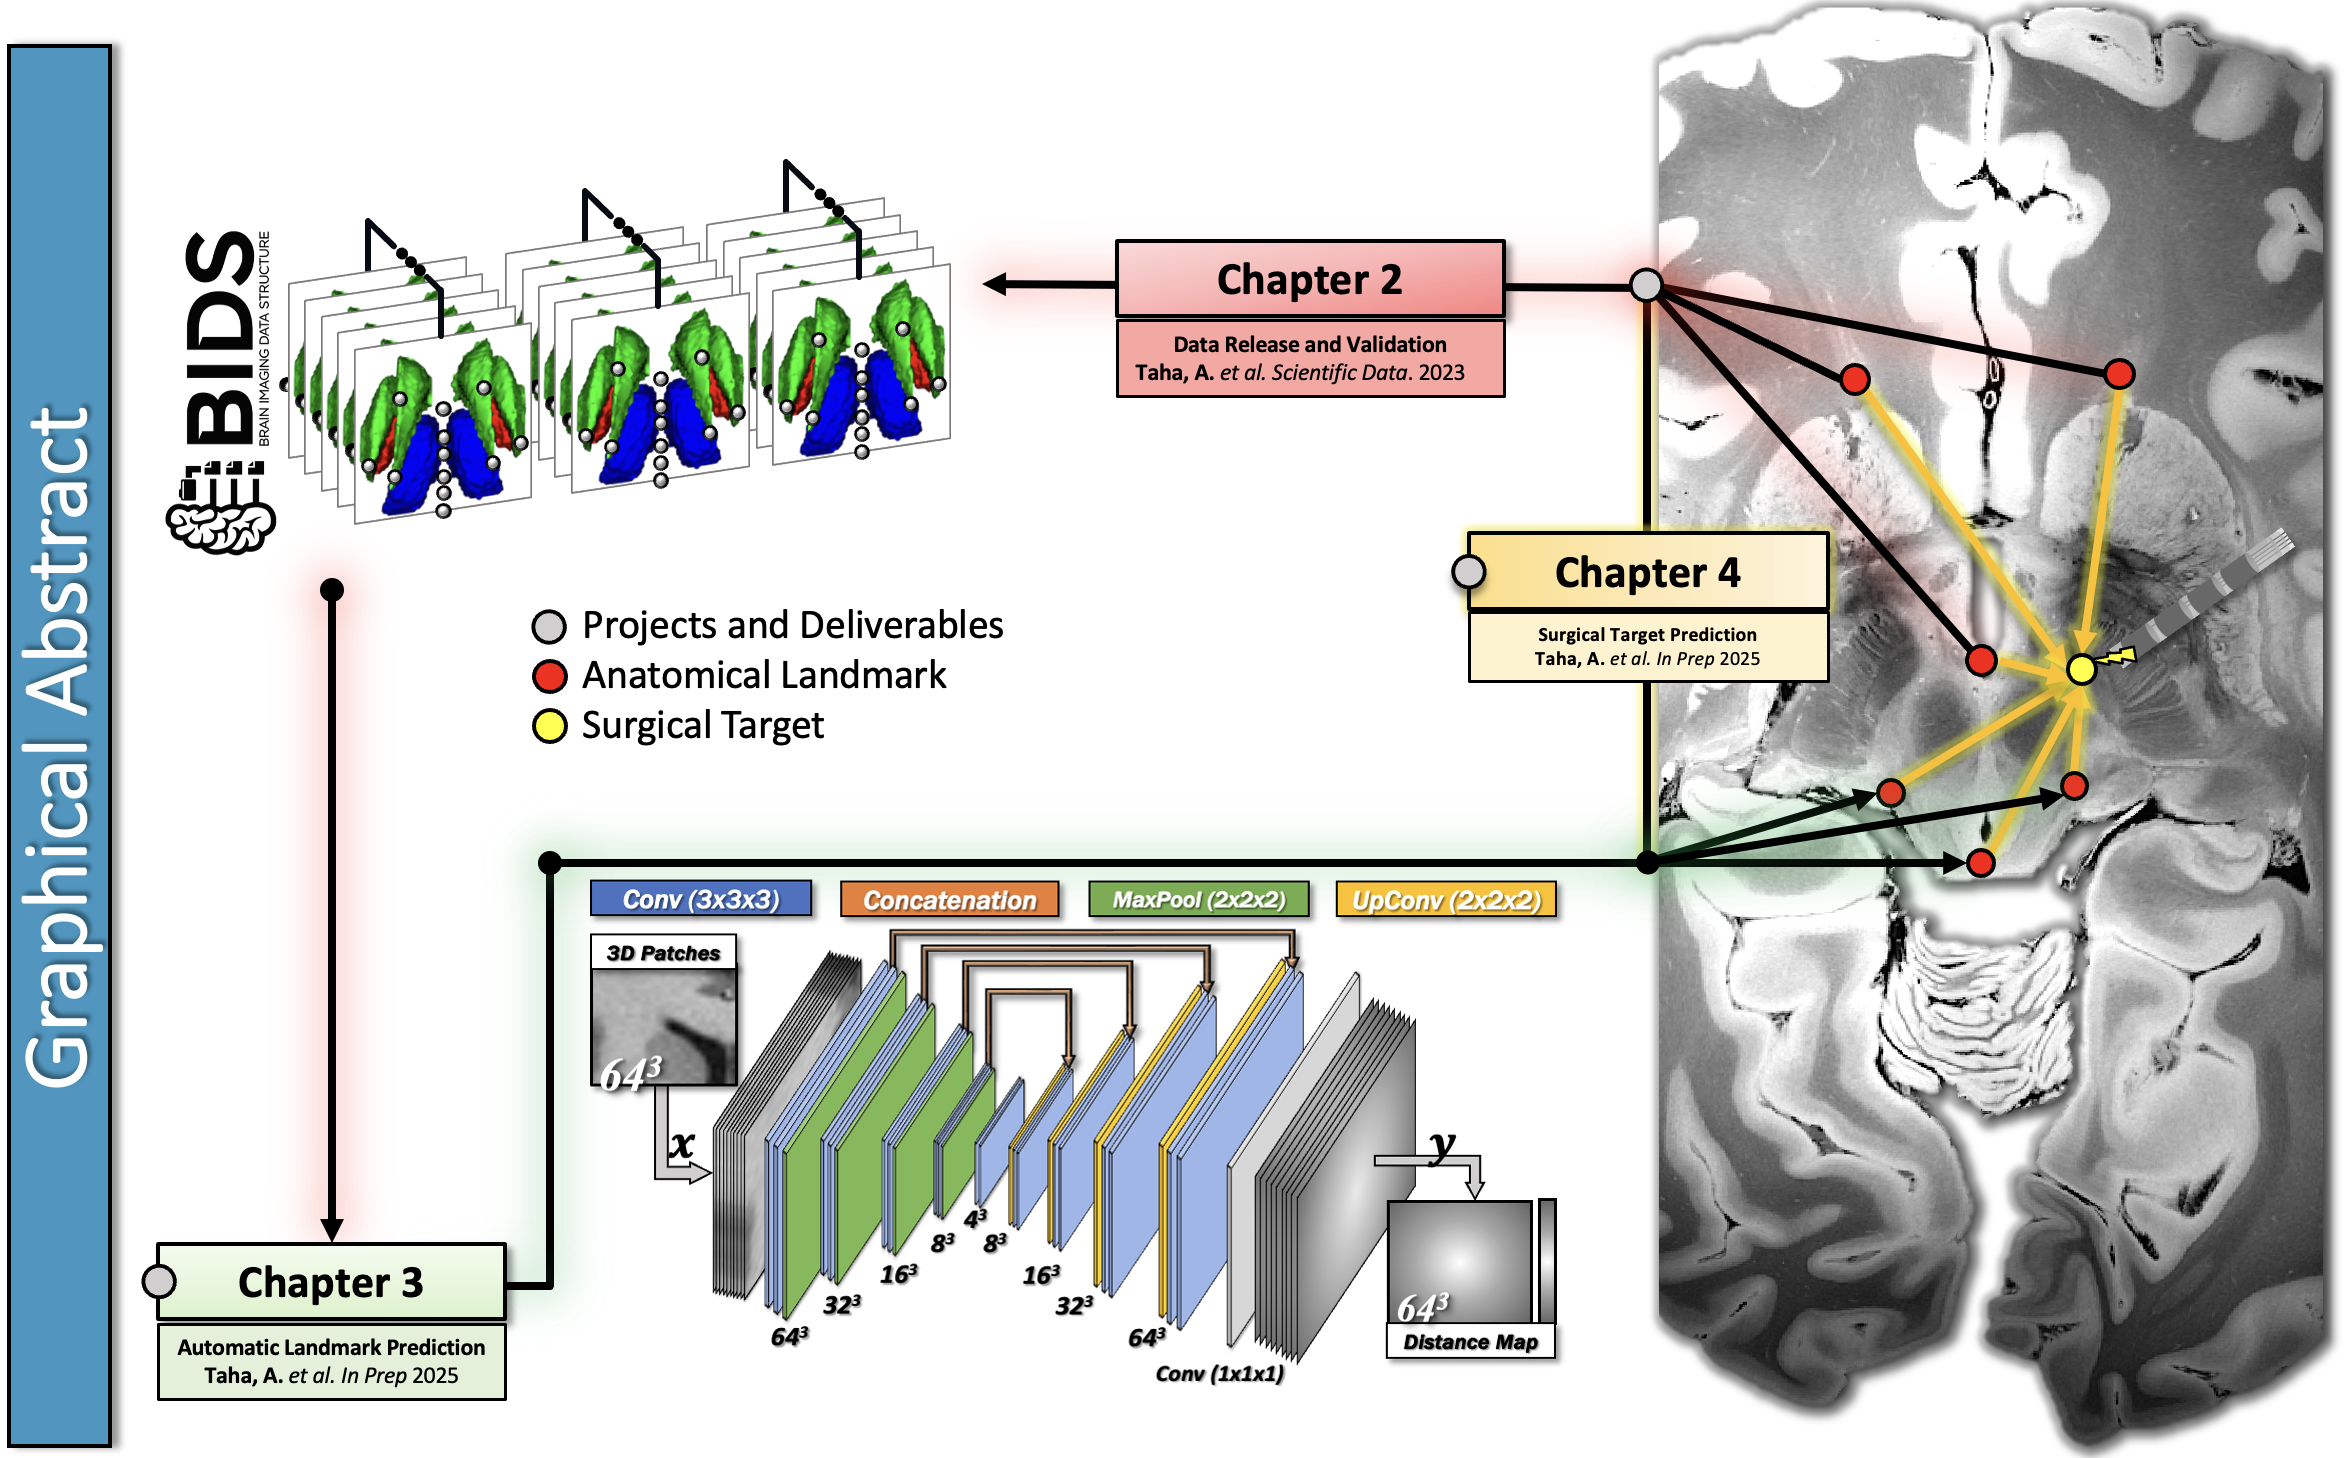
\includegraphics[width=1\linewidth]{figs/ch1_Figure_Abstract2.png}
    \caption{Graphical abstract of dissertation projects. \textit{Chapter 2} is focused on validation of a brain landmark annotation protocol and open release of data. \textit{Chapter 3} employs deep learning to automatically localize brain landmarks in an open-source implementation. \textit{Chapter 4} is focused on leveraging data and models from prior chapters to solve the deep brain stimulation target localization problem.}
    \label{fig:Abstract}
\end{figure}


This dissertation introduces a coordinate-based framework inspired by classical stereotactic principles and enhanced by modern machine learning to support spatially precise and interpretable workflows in neuroimaging and neurosurgery (Figure \ref{fig:Abstract}). We demonstrate how brain coordinates can be used to improve quality control and brain mapping in \textit{Chapter 2}, automate anatomical landmark detection in \textit{Chapter 3}, and predict the location of deep brain targets on clinical MRI in \textit{Chapter 4}. Together, these tools support surgical targeting and reliable population-level analyses. The specific objectives of each chapter are as follows:
\begin{itemize}
\item \textbf{\textit{Chapter 2}}: Validation of the Anatomical Fiducials (AFIDs) protocol—a standardized set of 32 anatomical landmarks—on multi-resolution structural MRI and the open release of annotated AFID datasets to support reproducibility and benchmarking.
\item \textbf{\textit{Chapter 3}}: Development of a modular, open-source pipeline for automatic AFID placement using machine learning with accuracy competitive to that of human raters.
\item \textbf{\textit{Chapter 4}}: Leverage AFID-derived geometry to predict the location of surgical targets and validate model generalizability across MRI modalities and field strengths.
\end{itemize}